% Chapter X

\chapter{Validation of the Heat Flux Partitioning Model} % Chapter title

\label{ch:HFP_validation} % For referencing the chapter elsewhere, use \autoref{ch:name} 

%----------------------------------------------------------------------------------------

In this Chapter, we want to assess the validity of the new Heat Flux Partitioning formulation proposed in Chapter \ref{chap:HFP_closures}. To do so, we will conduct two different validations:

\begin{itemize}
\setlength{\itemsep}{8pt}
\item The first part will be dedicated to validation on a single experimental subcooled boiling case at 10.5 bar from Kossolapov \cite{kossolapov_experimental_2021} for which numerous physical parameters have been measured. This will ensure that the mathematical formulation and the closure laws propose an acceptable physical modeling of the boiling parameters.

\item The second part will consist on wall temperature predictions for vertical subcooled flow boiling of water in various conditions, including pressure. Experimental database from Jens \& Lottes \cite{jens_analysis_1951}, Kennel \cite{kennel_local_1949} and Kossolapov \cite{kossolapov_experimental_2021}. Comparison with other HFP models from Kurul \& Podowski, Basu and Kommajosyula will be performed.
\end{itemize}


\section{Detailed Comparison and Assessment of the Heat Flux Partitioning}

In this section, we compare our results to those obtaines by Kossolapov \cite{kossolapov_experimental_2021} in vertical subcooled flow boiling. At a pressure of 10.5 bar, he realized measurements of many relevant parameters regarding the Heat Flux Partitioning:

\begin{itemize}
\item Active nucleation site density $N_{sit,a}$ ;
\item Bubble nucleation frequency $f$ ;
\item Bubble wait time $t_{w}$ ;
\item Transient heat transfer (quenching) time $t_{q}$ ;
\item Average bubble growth time $t_{g}$ ;
\item Average area visited by a bubble $A_{q,1b}$ ;
\item Proportion of the heater area impacted by bubbles $A_{b,tot}$
\item Liquid single-phase heat flux proportion $\dfrac{\phi_{c,L}}{\phi_{w}}$ ;
\item Quenching heat flux proportion $\dfrac{\phi_{q}}{\phi_{w}}$ ;
\item Wall superheat $\Delta T_{w}$.
\end{itemize}

The only lacking parameters to conduct a full evaluation of the model would be the average bubble departure diameter $R_{d}$, sliding length $l_{sl}$ and lift-off diameter / coalescence diameter.

The values provided by Kossolapov are an average conducted over all the observed nucleation events during the time of the experiment. Such data are representative of what we want to achieve using a HFP model since we represent average values of the boiling parameters for the considered boiling surface.

\npar

All those variables were measured for a subcooling $\Delta T_{L} = 10\degC$ at three different liquid mass fluxes $G_{L} = 500$, $1000$ and $2000~\debm$. 

\npar

We present the results obtained by comparison with the case at $G_{L} = 2000\ \debm$ for each variable. The simulations using the HFP model were conducted using a contact angle $\theta = 85 \degree$ (usual contact angle for water and ITO \cite{kossolapov_experimental_2021}), an hysteresis $\dtheta = 2 \degree$ and a growth constant $K=0.8$

 
\subsection{Active Nucleation Site Density}

On Figure \ref{fig:fullkoss_nsit}, we compare the values obtained for the active nucleation site density. The Li \etal correlation used in the model (Eq. \ref{eq:nsit_li}) propose a reasonable prediction of the measured values of $N_{sit,a}$ with an underestimation of less than a decade. The correlation correctly reproduce the experimental trend where we observe a sort of saturation in the nucleation site density for higher wall superheat.

\npar

To better match the asymptotic value of the experiment, we correct the Li \etal correlation for this case by a factor $\Delta T_{w}^{2-0.3\Delta T_{w}^{0.5}}$ which better fits the measurements for $\Delta T_{w}>10$~K but yields a small overestimation before.


\begin{figure}[!h]
\subfloat[$N_{sit,a}$ predictions by Li \etal correlation]{
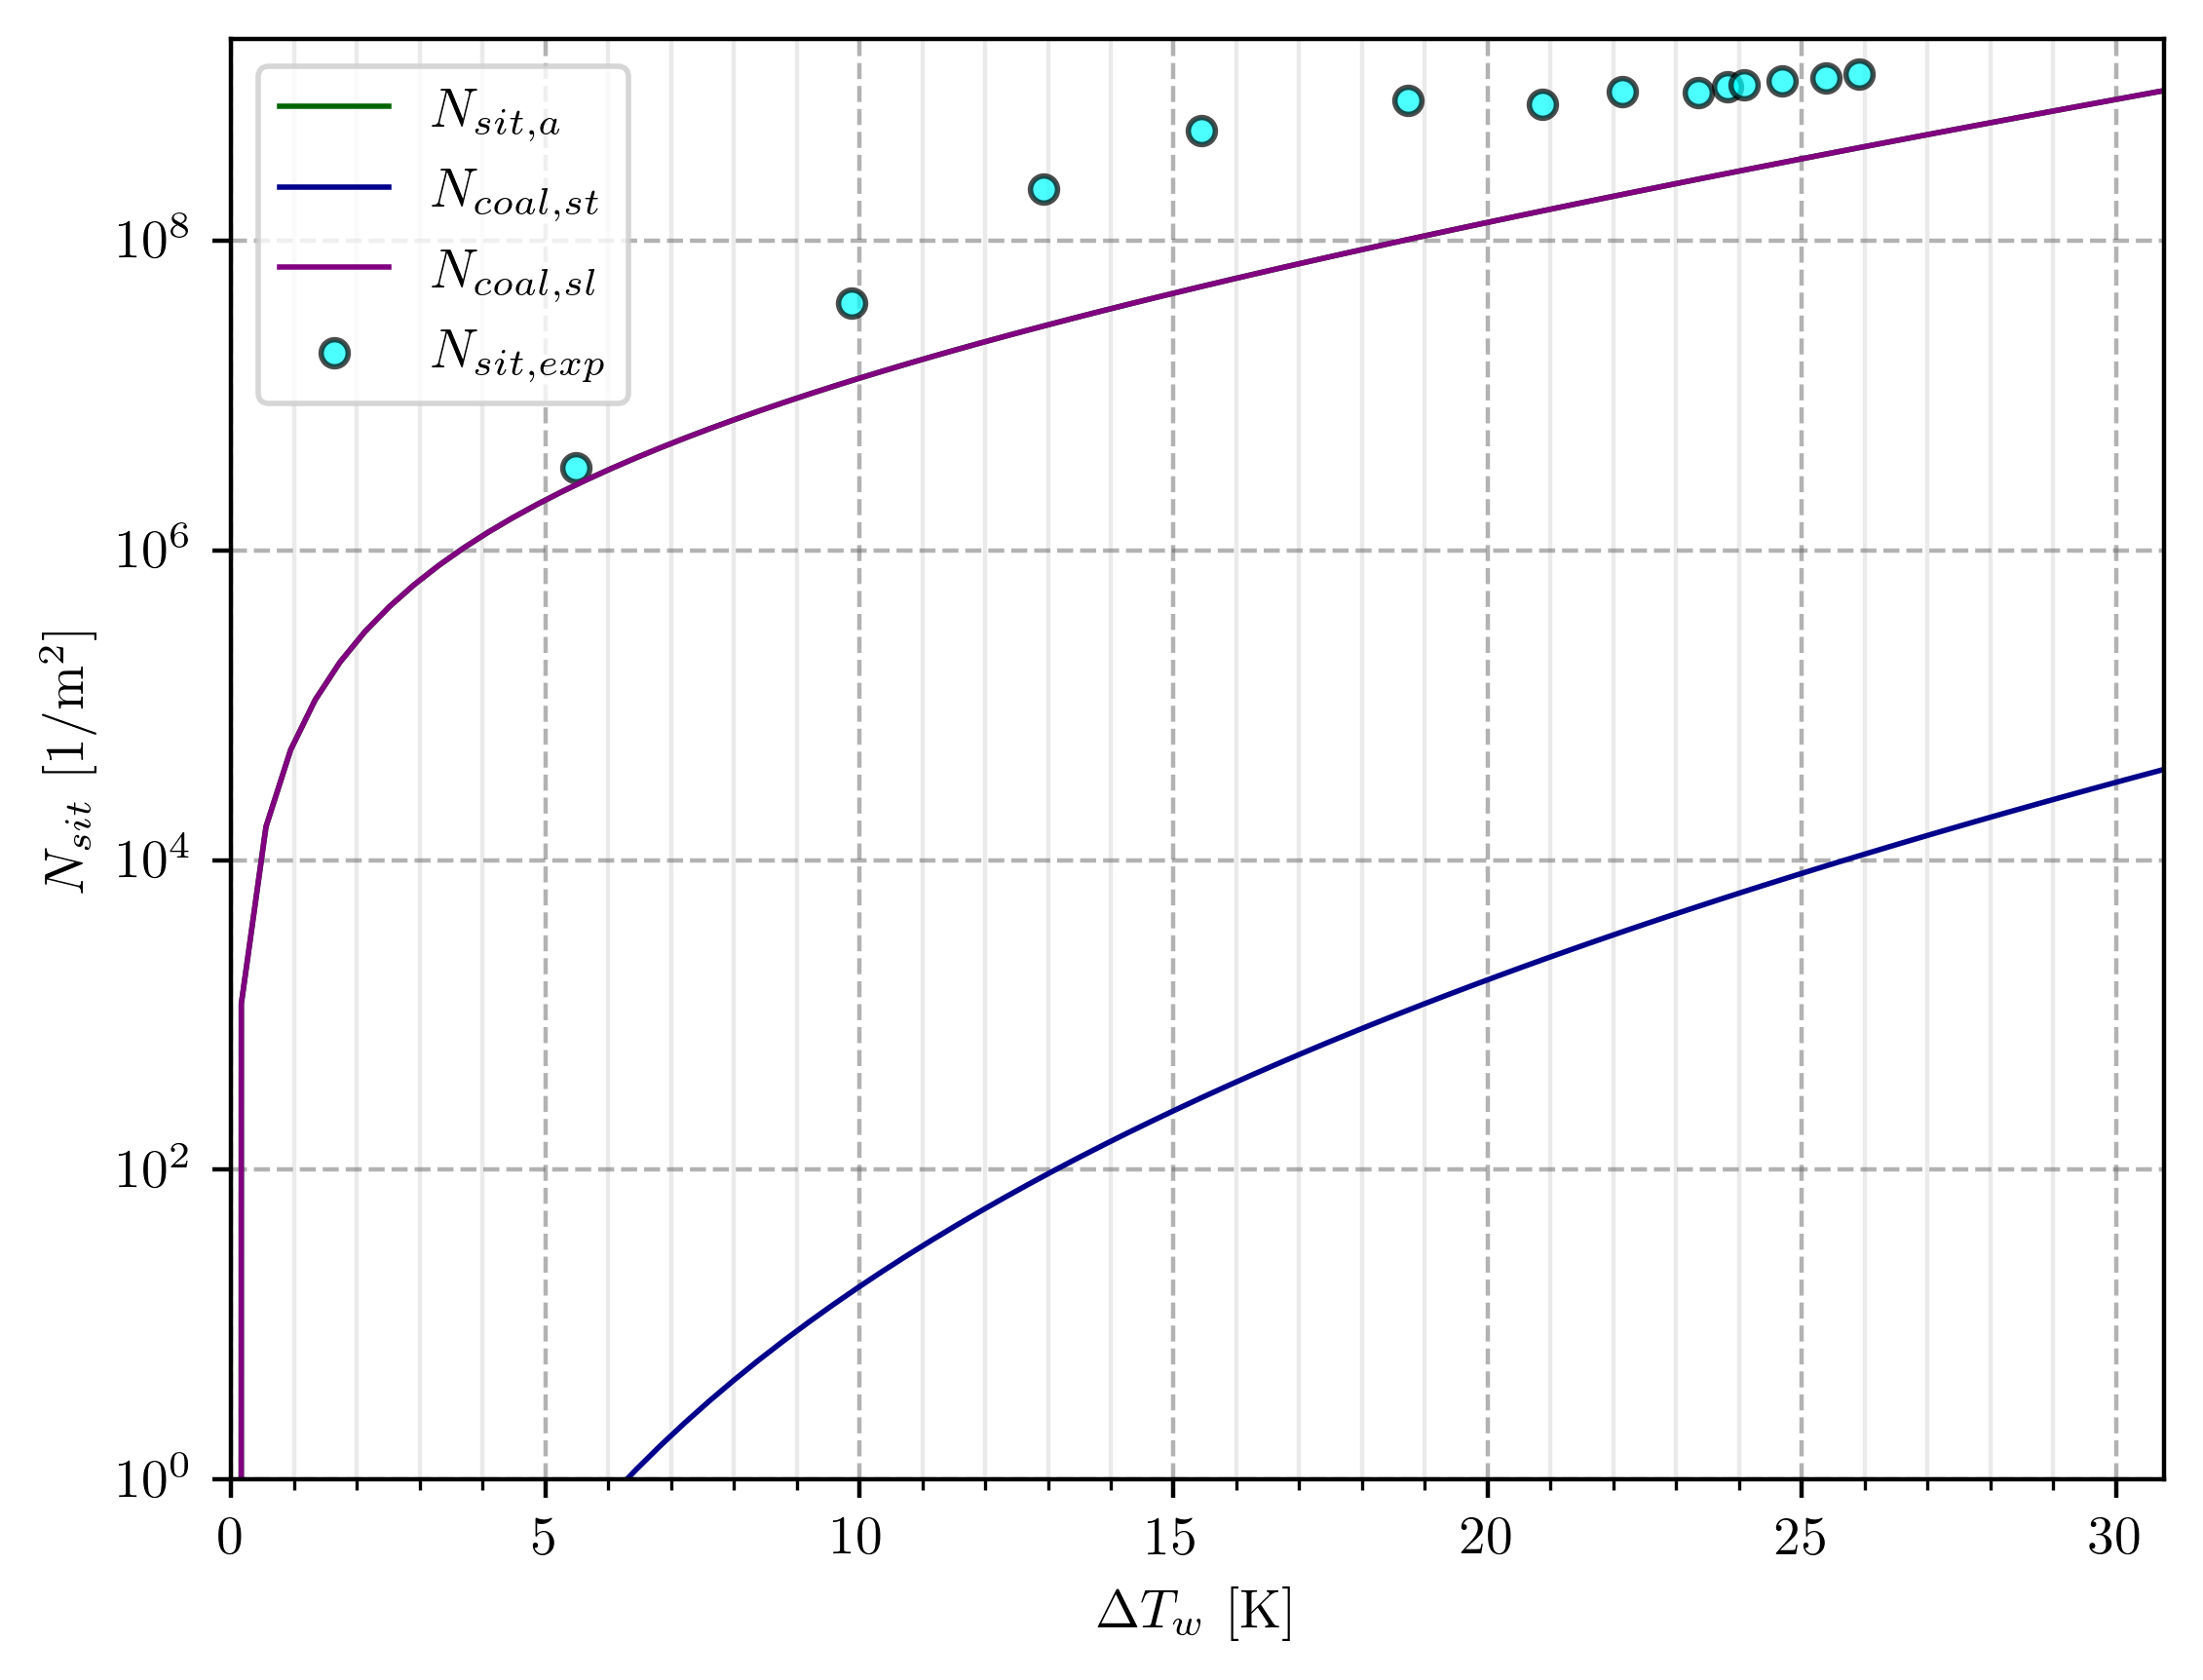
\includegraphics[width=0.5\linewidth]{img/HFP/fullcomp_Koss/sites_G2000_nocorr.png}
}
\subfloat[$N_{sit,a}$ predictions with corrected Li \etal correlation]{
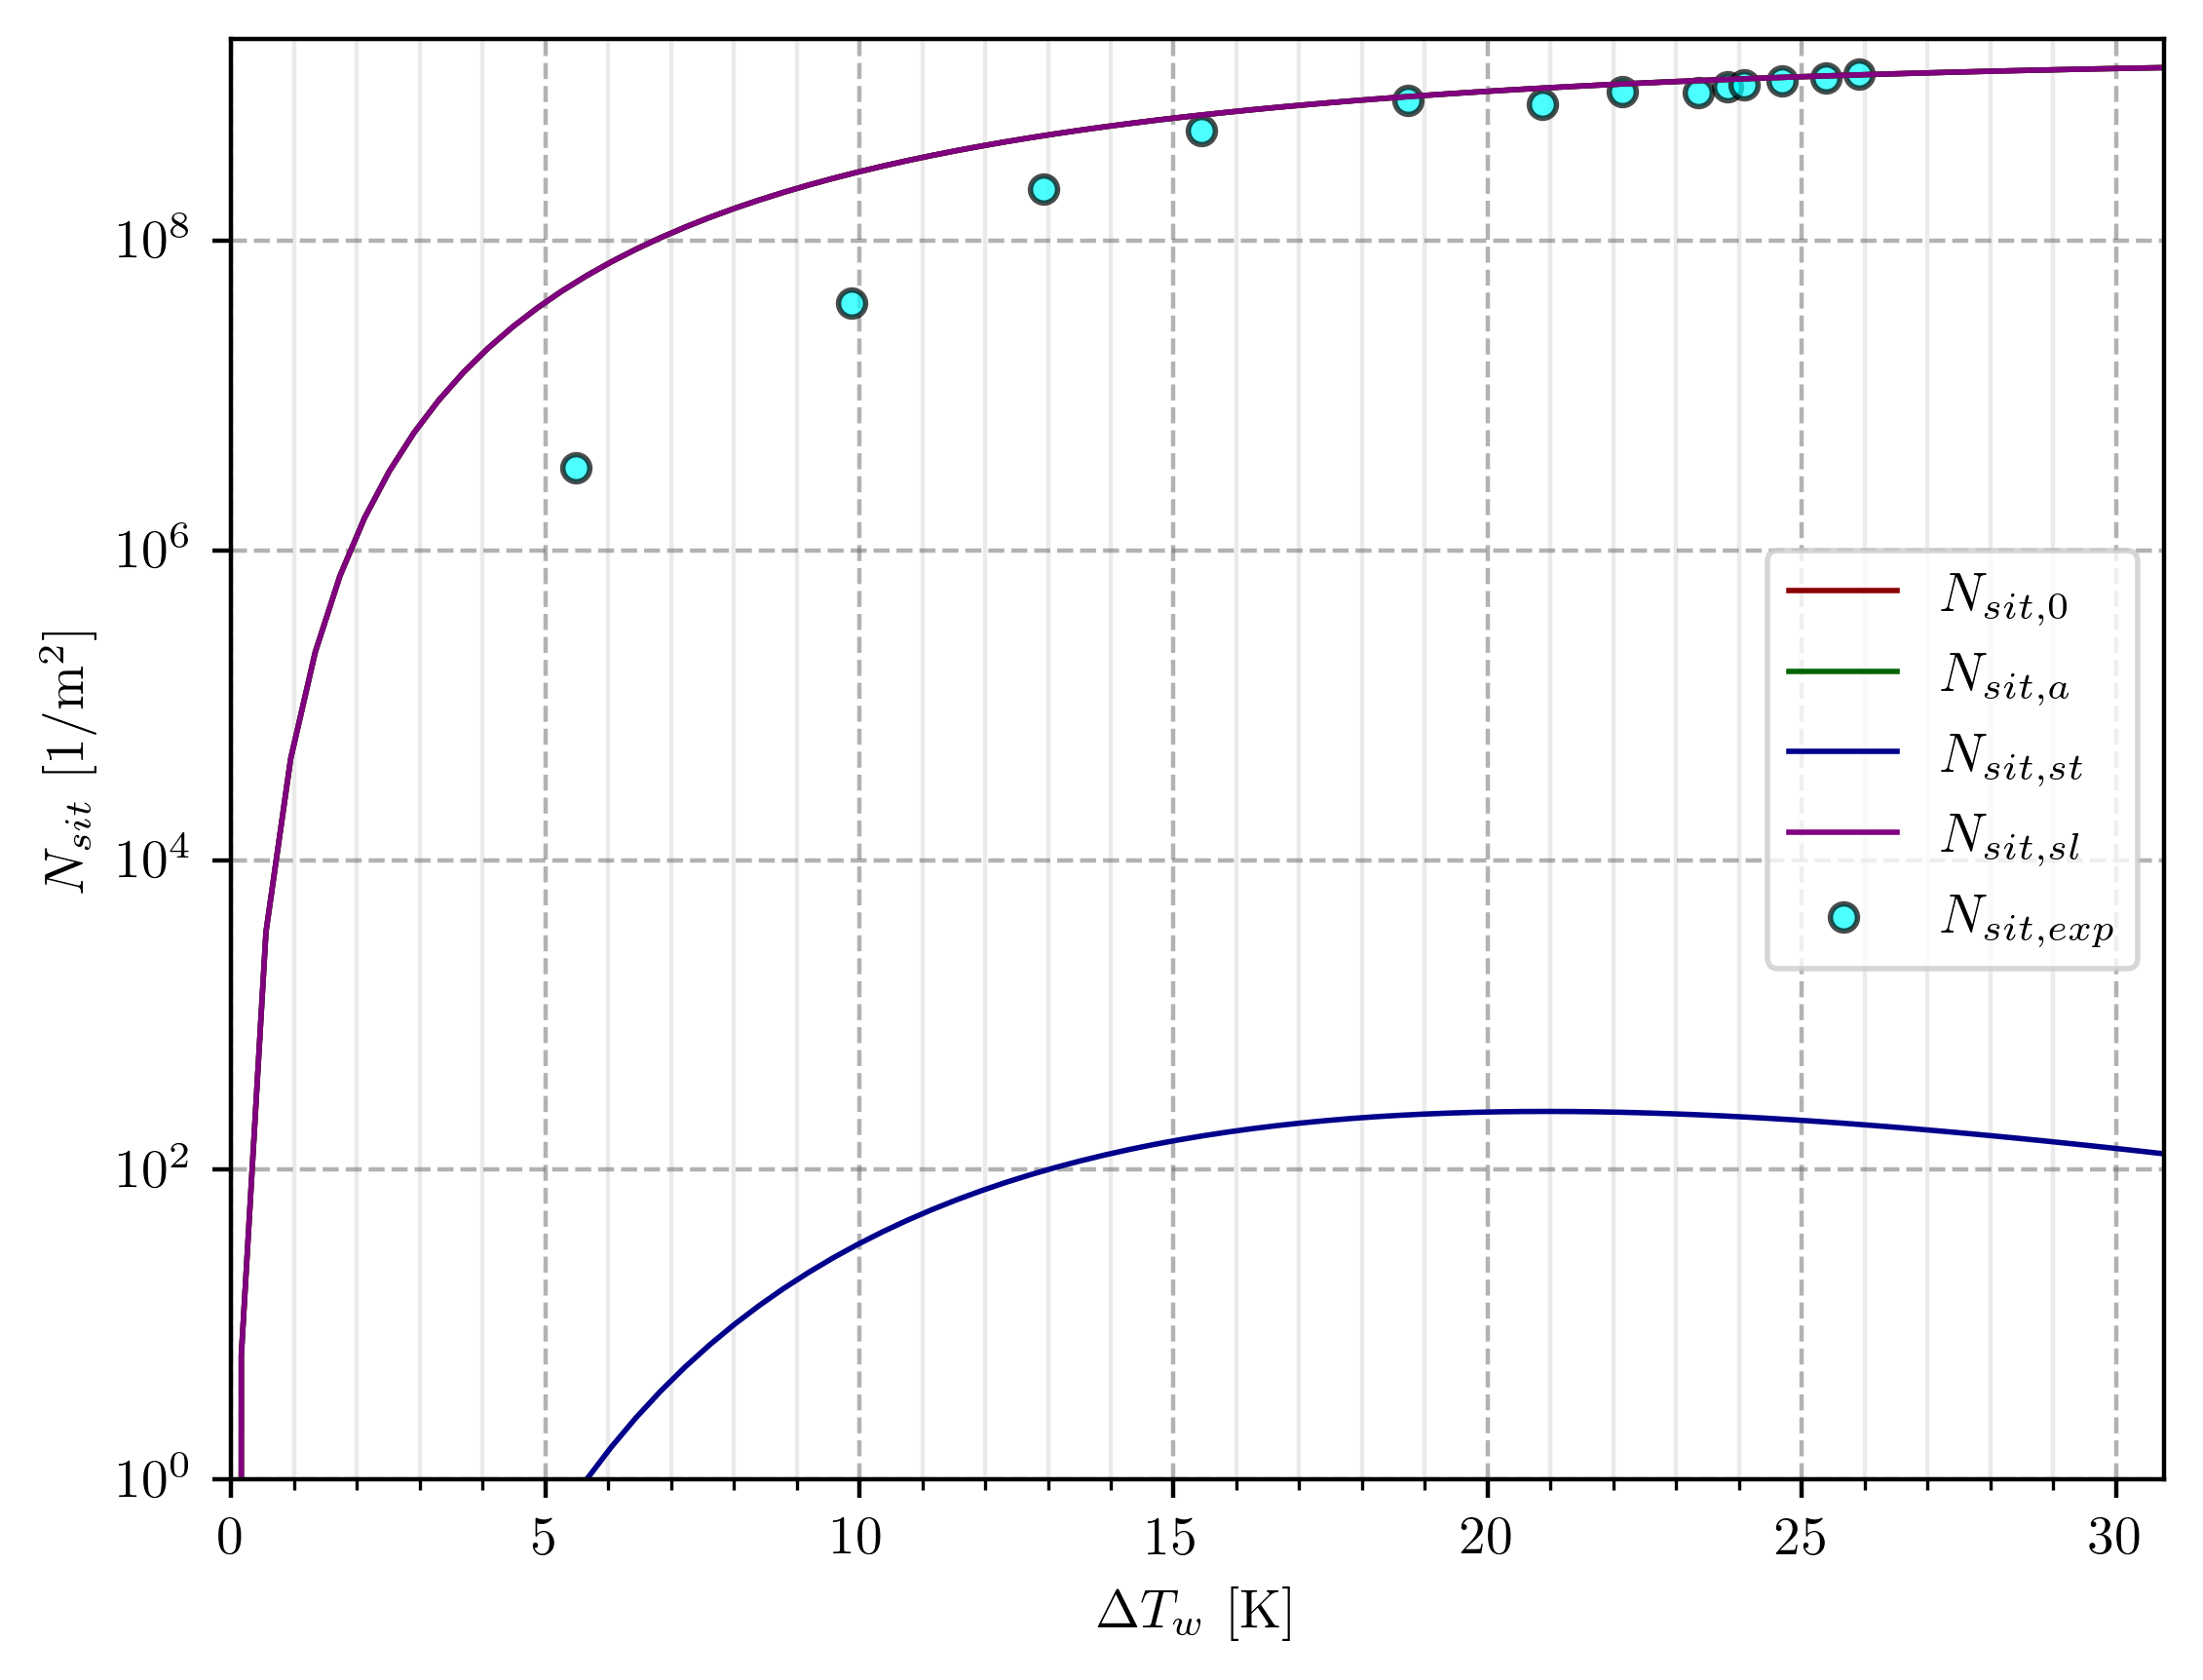
\includegraphics[width=0.5\linewidth]{img/HFP/fullcomp_Koss/sites_G2000.png}
}
\caption{Comparison of active nucleation site density with and without a correction for Li \etal formulation.}
\label{fig:fullkoss_nsit}
\end{figure}



\begin{note*}{}
Following comparisons are conducted using the corrected value of $N_{sit,a}$ to limit the impact of the nucleation site density prediction over the other parameters.
\end{note*}

\subsection{Wait Time, Growth Time, Quenching Time and Nucleation Frequency}

Figure \ref{fig:fullkoss_times} compares the different times involved in the boiling physics and the bubble nucleation frequency. As seen in Section \ref{sec:wait_time}, the wait time is quite fairly reproduced along with the nucleation frequency. Actually, the bubble departure is nearly instantaneous and the nucleation cycle is mainly composed of the wait period, which means a good estimation of $t_{w}$ leads to a reasonable estimation of $f$ for this case.

\npar

The average bubble growth time is overestimated by nearly a decade for low superheat and is better predicted for larger superheat. Its evolution seem coherent with a decrease up to 15\ K and a stabilization afterwards. However, the experimental measurements show an increase in the growth time for large superheat which could be associated to bubble diameter increase with the wall Jakob number as previously observed in Section \ref{sec:liftoff}. This could be in partial contradiction with the single coalescence hypothesis for the lift-off since the average distance between bubbles in likely to decrease with wall superheat, thus decreasing the average growth time. On the other hand, the growth time overprediction may be associated to sliding length overestimation.

\npar

A very good approximation of the quenching time $t_{q}$ is achieved using the time $t^{*}$ (Eq. \ref{eq:tstar}). This indicates that for this experimental case, the large value of the wait time implies that the transient conduction will be limited to a duration $t^{*}$ and that the remaining wait time will be governed by forced convection. 

\begin{figure}[!h]
\subfloat[Bubble nucleation frequency]{
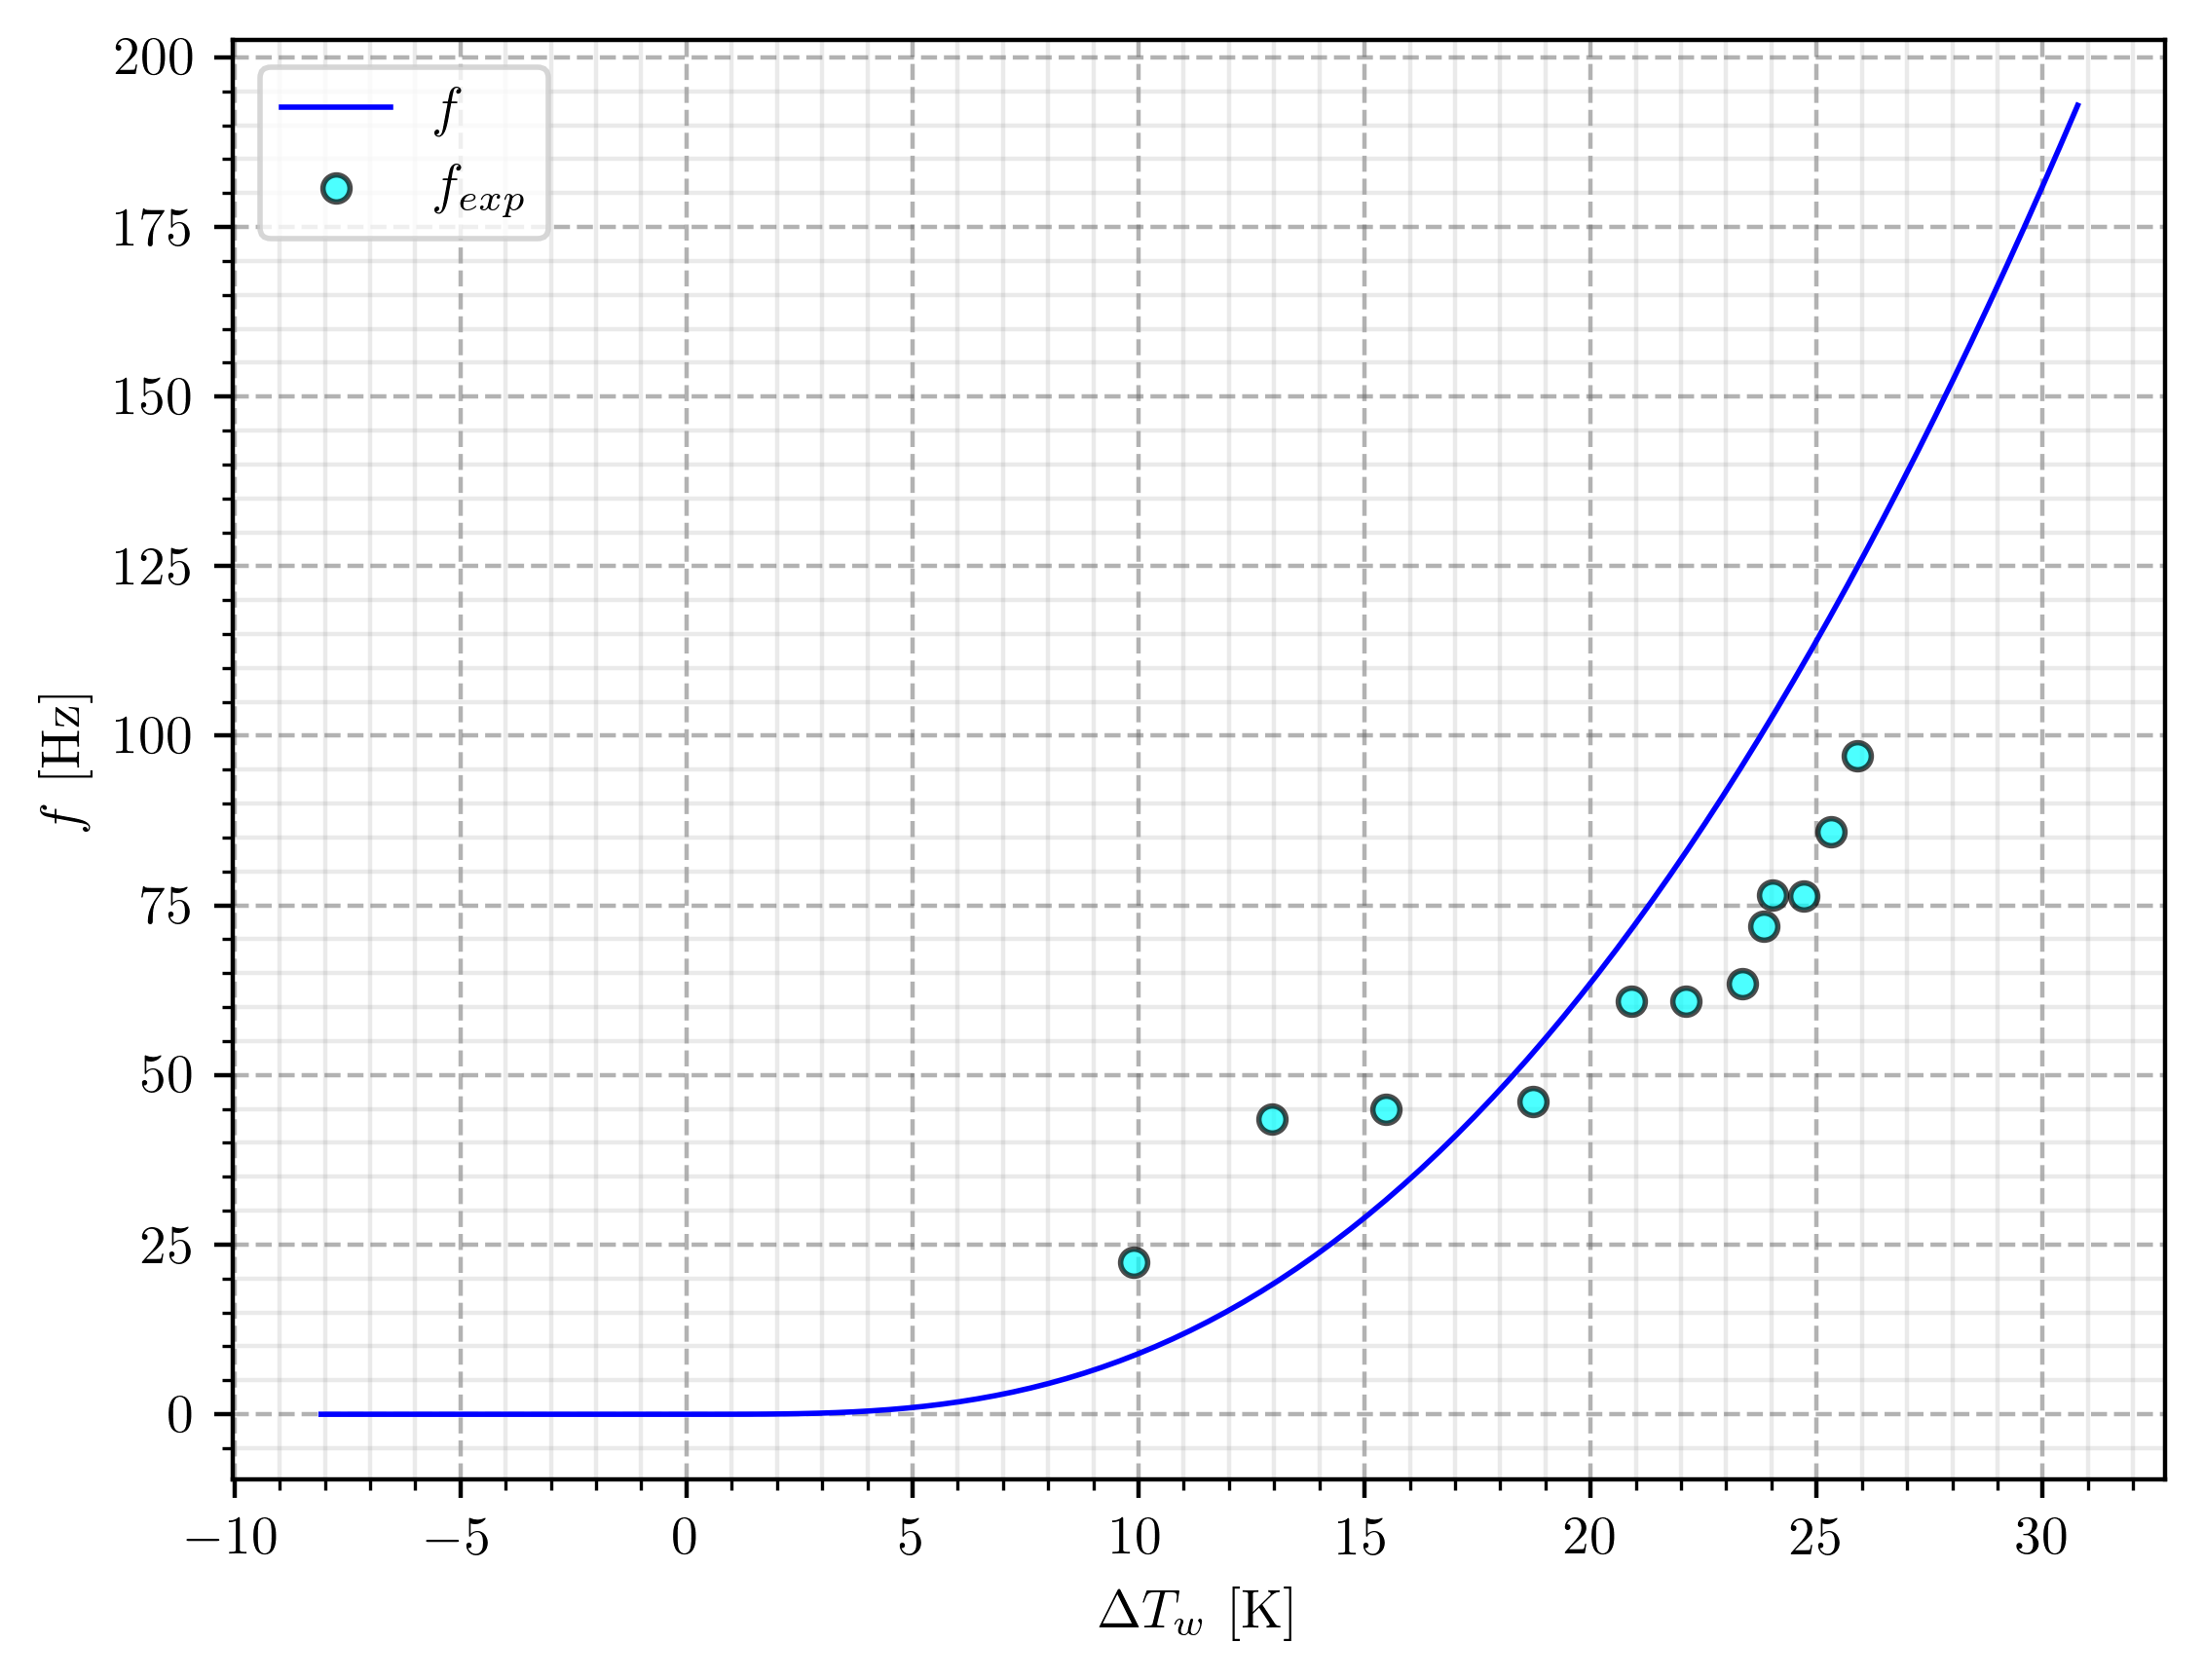
\includegraphics[width=0.5\linewidth]{img/HFP/fullcomp_Koss/f_G2000.png}
}
\subfloat[Bubble wait time, growth time and quenching time]{
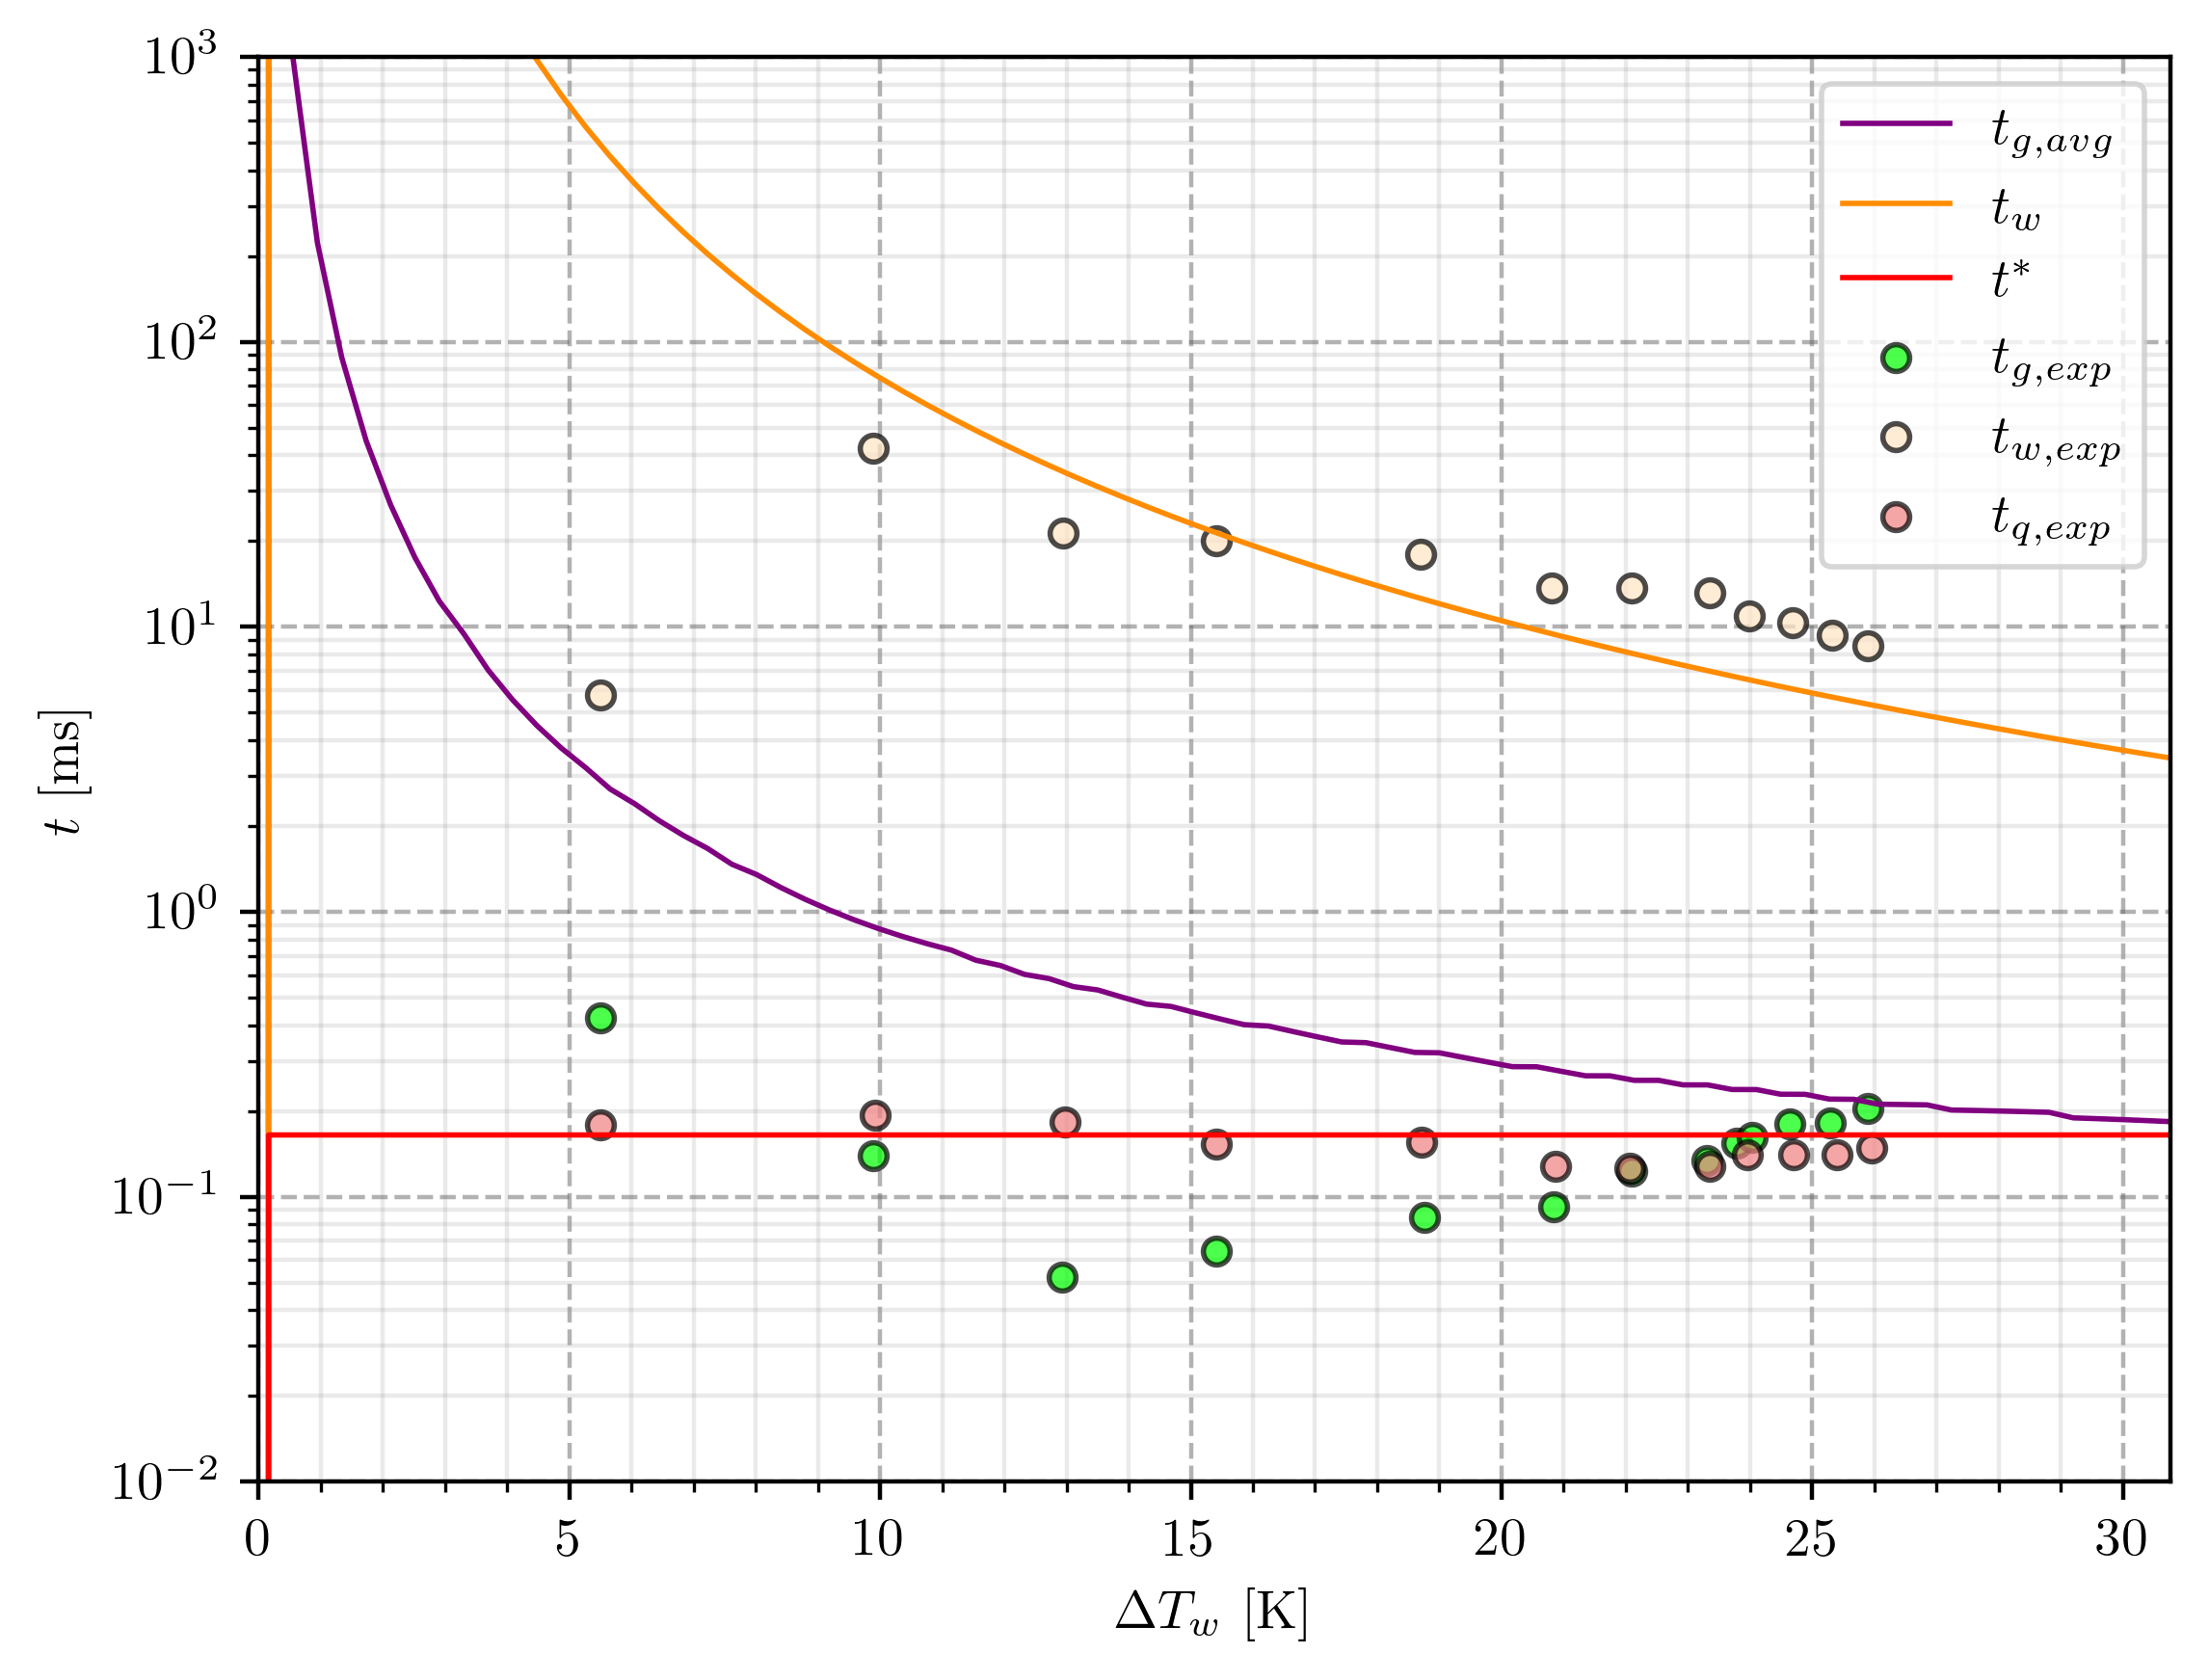
\includegraphics[width=0.5\linewidth]{img/HFP/fullcomp_Koss/times_G2000.png}
}
\caption{Comparison of bubble nucleation frequency, wait time, average growth time and quenching time.}
\label{fig:fullkoss_times}
\end{figure}





\subsection{Single Bubble Area and Total Bubble Area}

Figure \ref{fig:fullkoss_area} that the total area visited by a bubble is largely overestimated for the whole boiling curve. It only achieves a reasonable order of magnitude at high wall superheat ($\Delta T_{w} > 23\ $K). This could question the usual hypothesis that supposes a sliding length $l_{sl}$ equal to the average distance between bubbles $s_{b} = 0.5/\sqrt{N_{b}}$. The sole projected area of the bubbles is in average better for the visited area, but underpredicts the largest values of $A_{q,1b}$ when bubbles start sliding over significant lengths.

\npar

Moreover, both values do not reproduce the experimental trend where the visited area regularly increases with the wall superheat. Further experimental insights regarding the behavior of the bubble sliding length could allow a better modeling of $l_{sl}$ depending on the bubble lift-off process as discussed in Section \ref{sec:liftoff}.

\npar

Those results naturally lead to an overprediction of the wall area fraction impacted by bubbles but shows an coherent increasing trend with wall superheat.

\npar 



\begin{figure}[!h]
\subfloat[Single bubble area]{
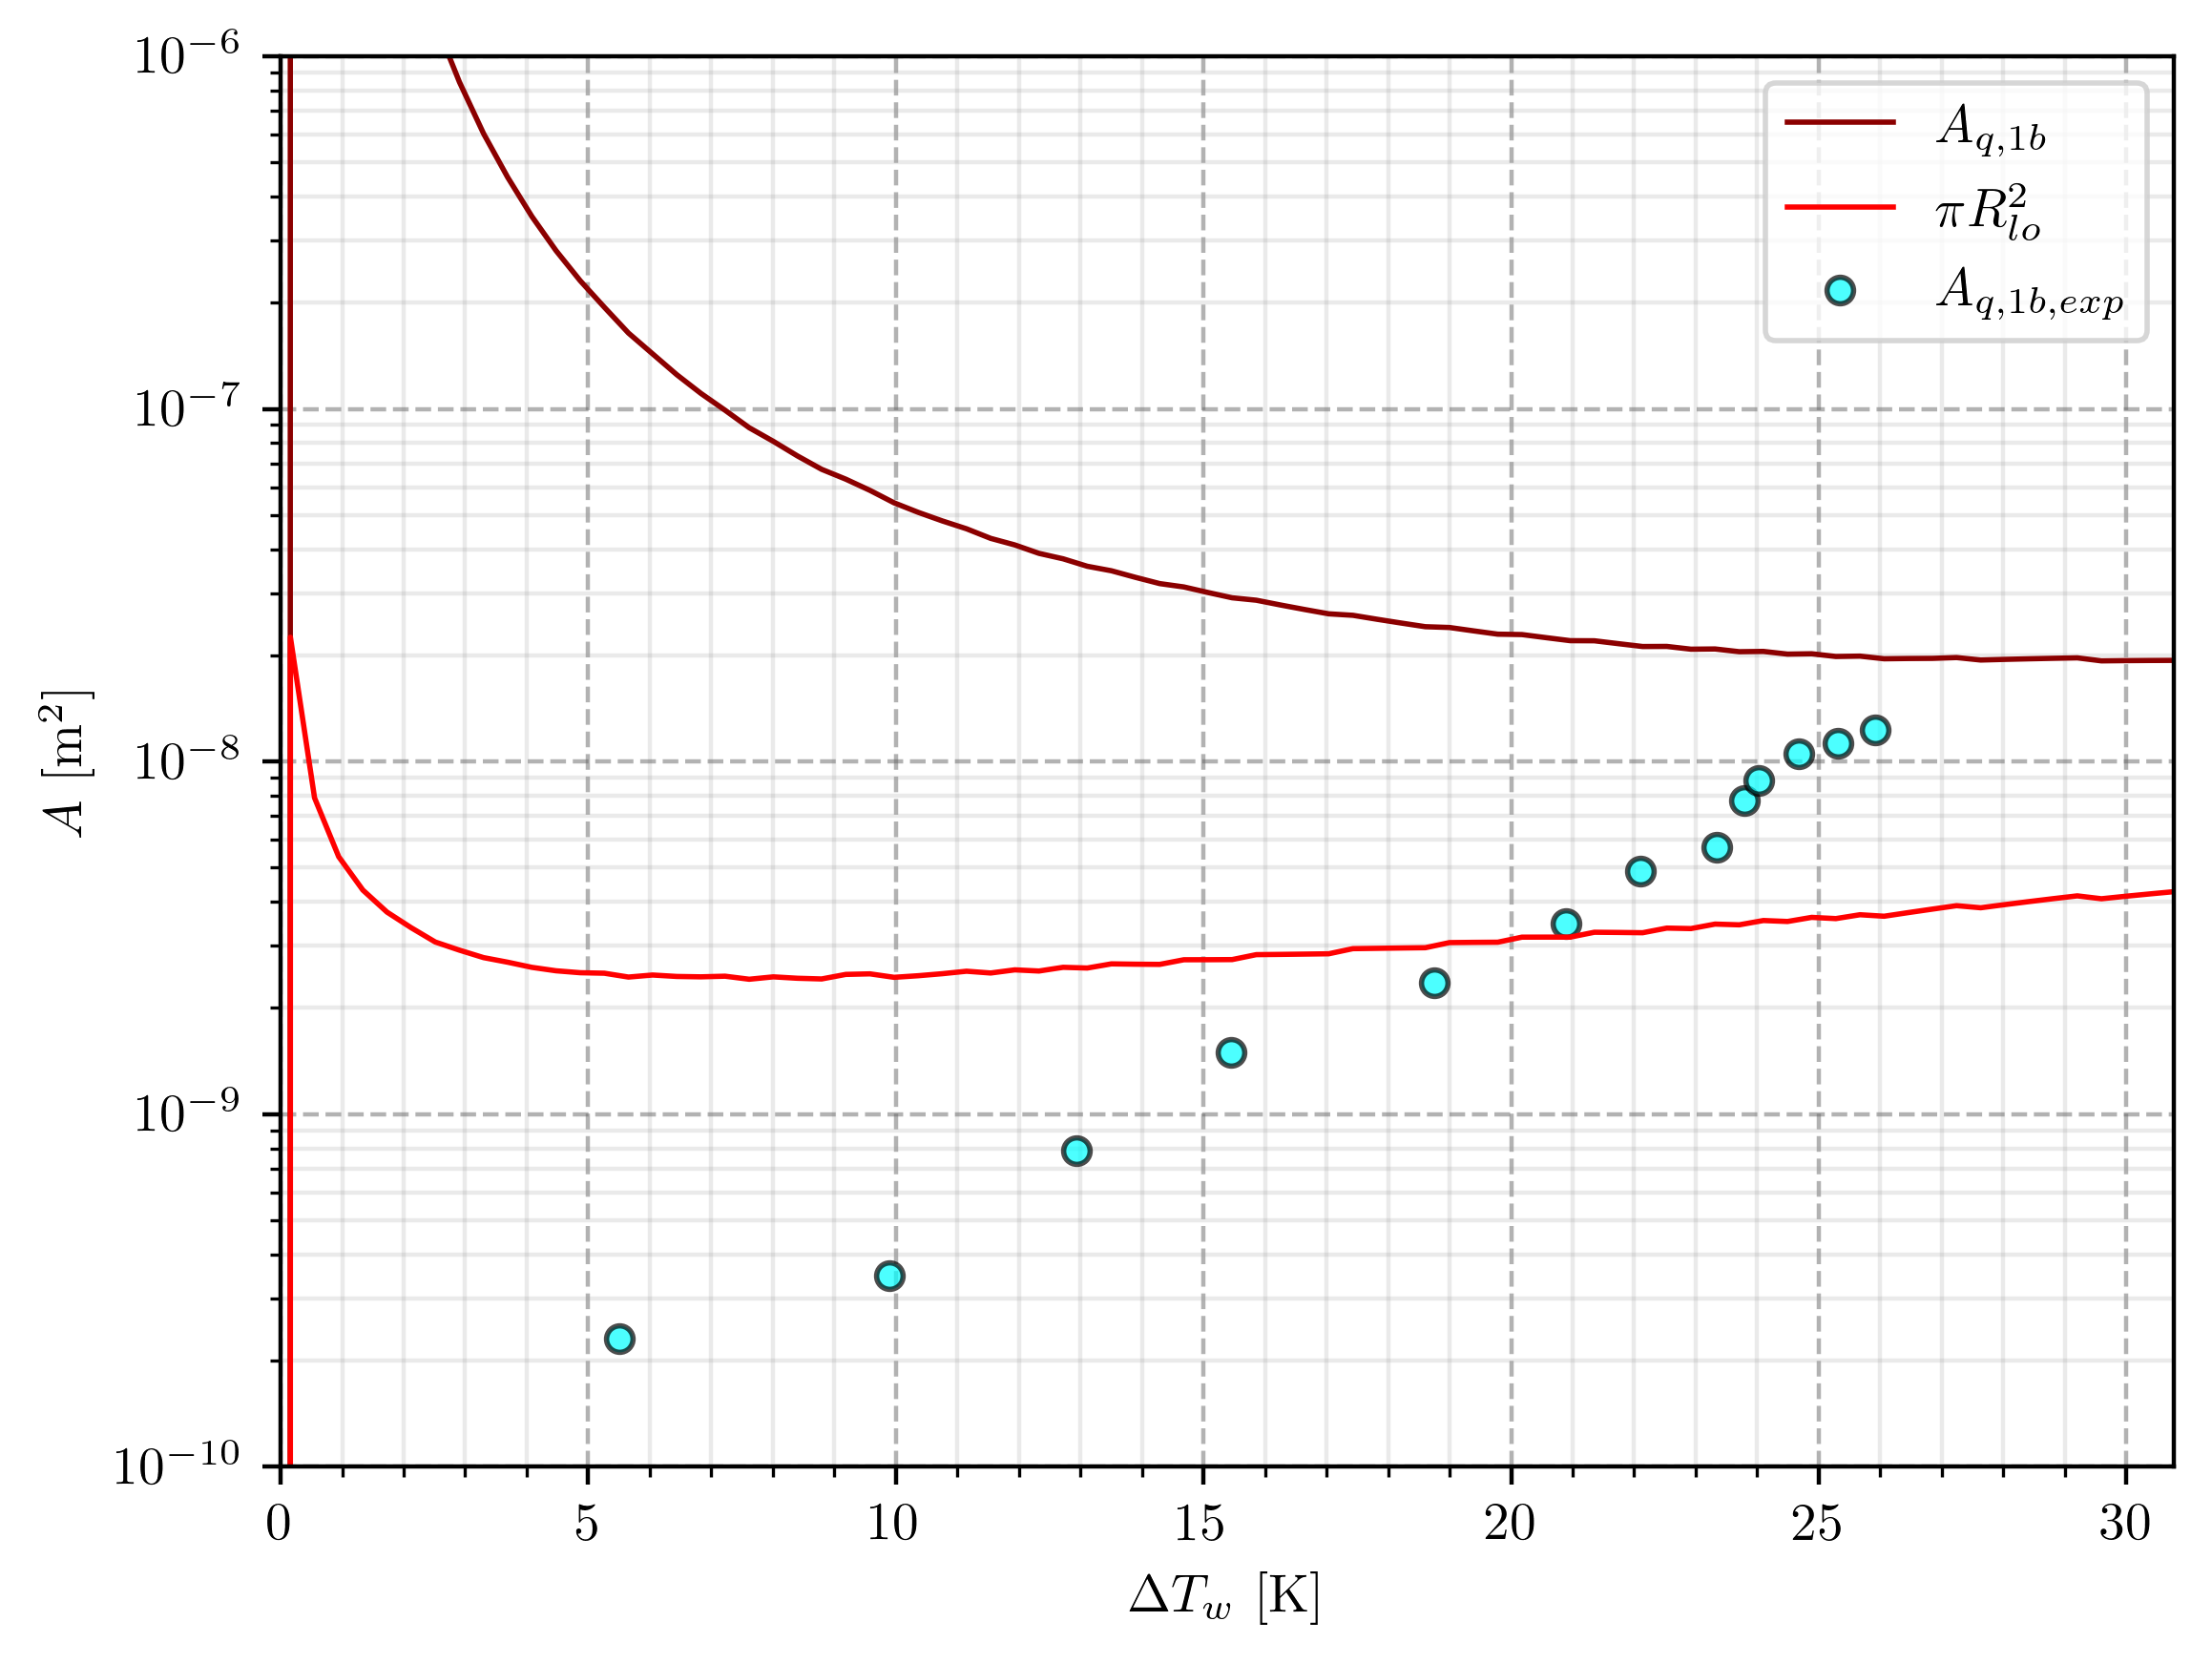
\includegraphics[width=0.5\linewidth]{img/HFP/fullcomp_Koss/Aq1b_G2000.png}
}
\subfloat[Total wall area impacted by bubbles]{
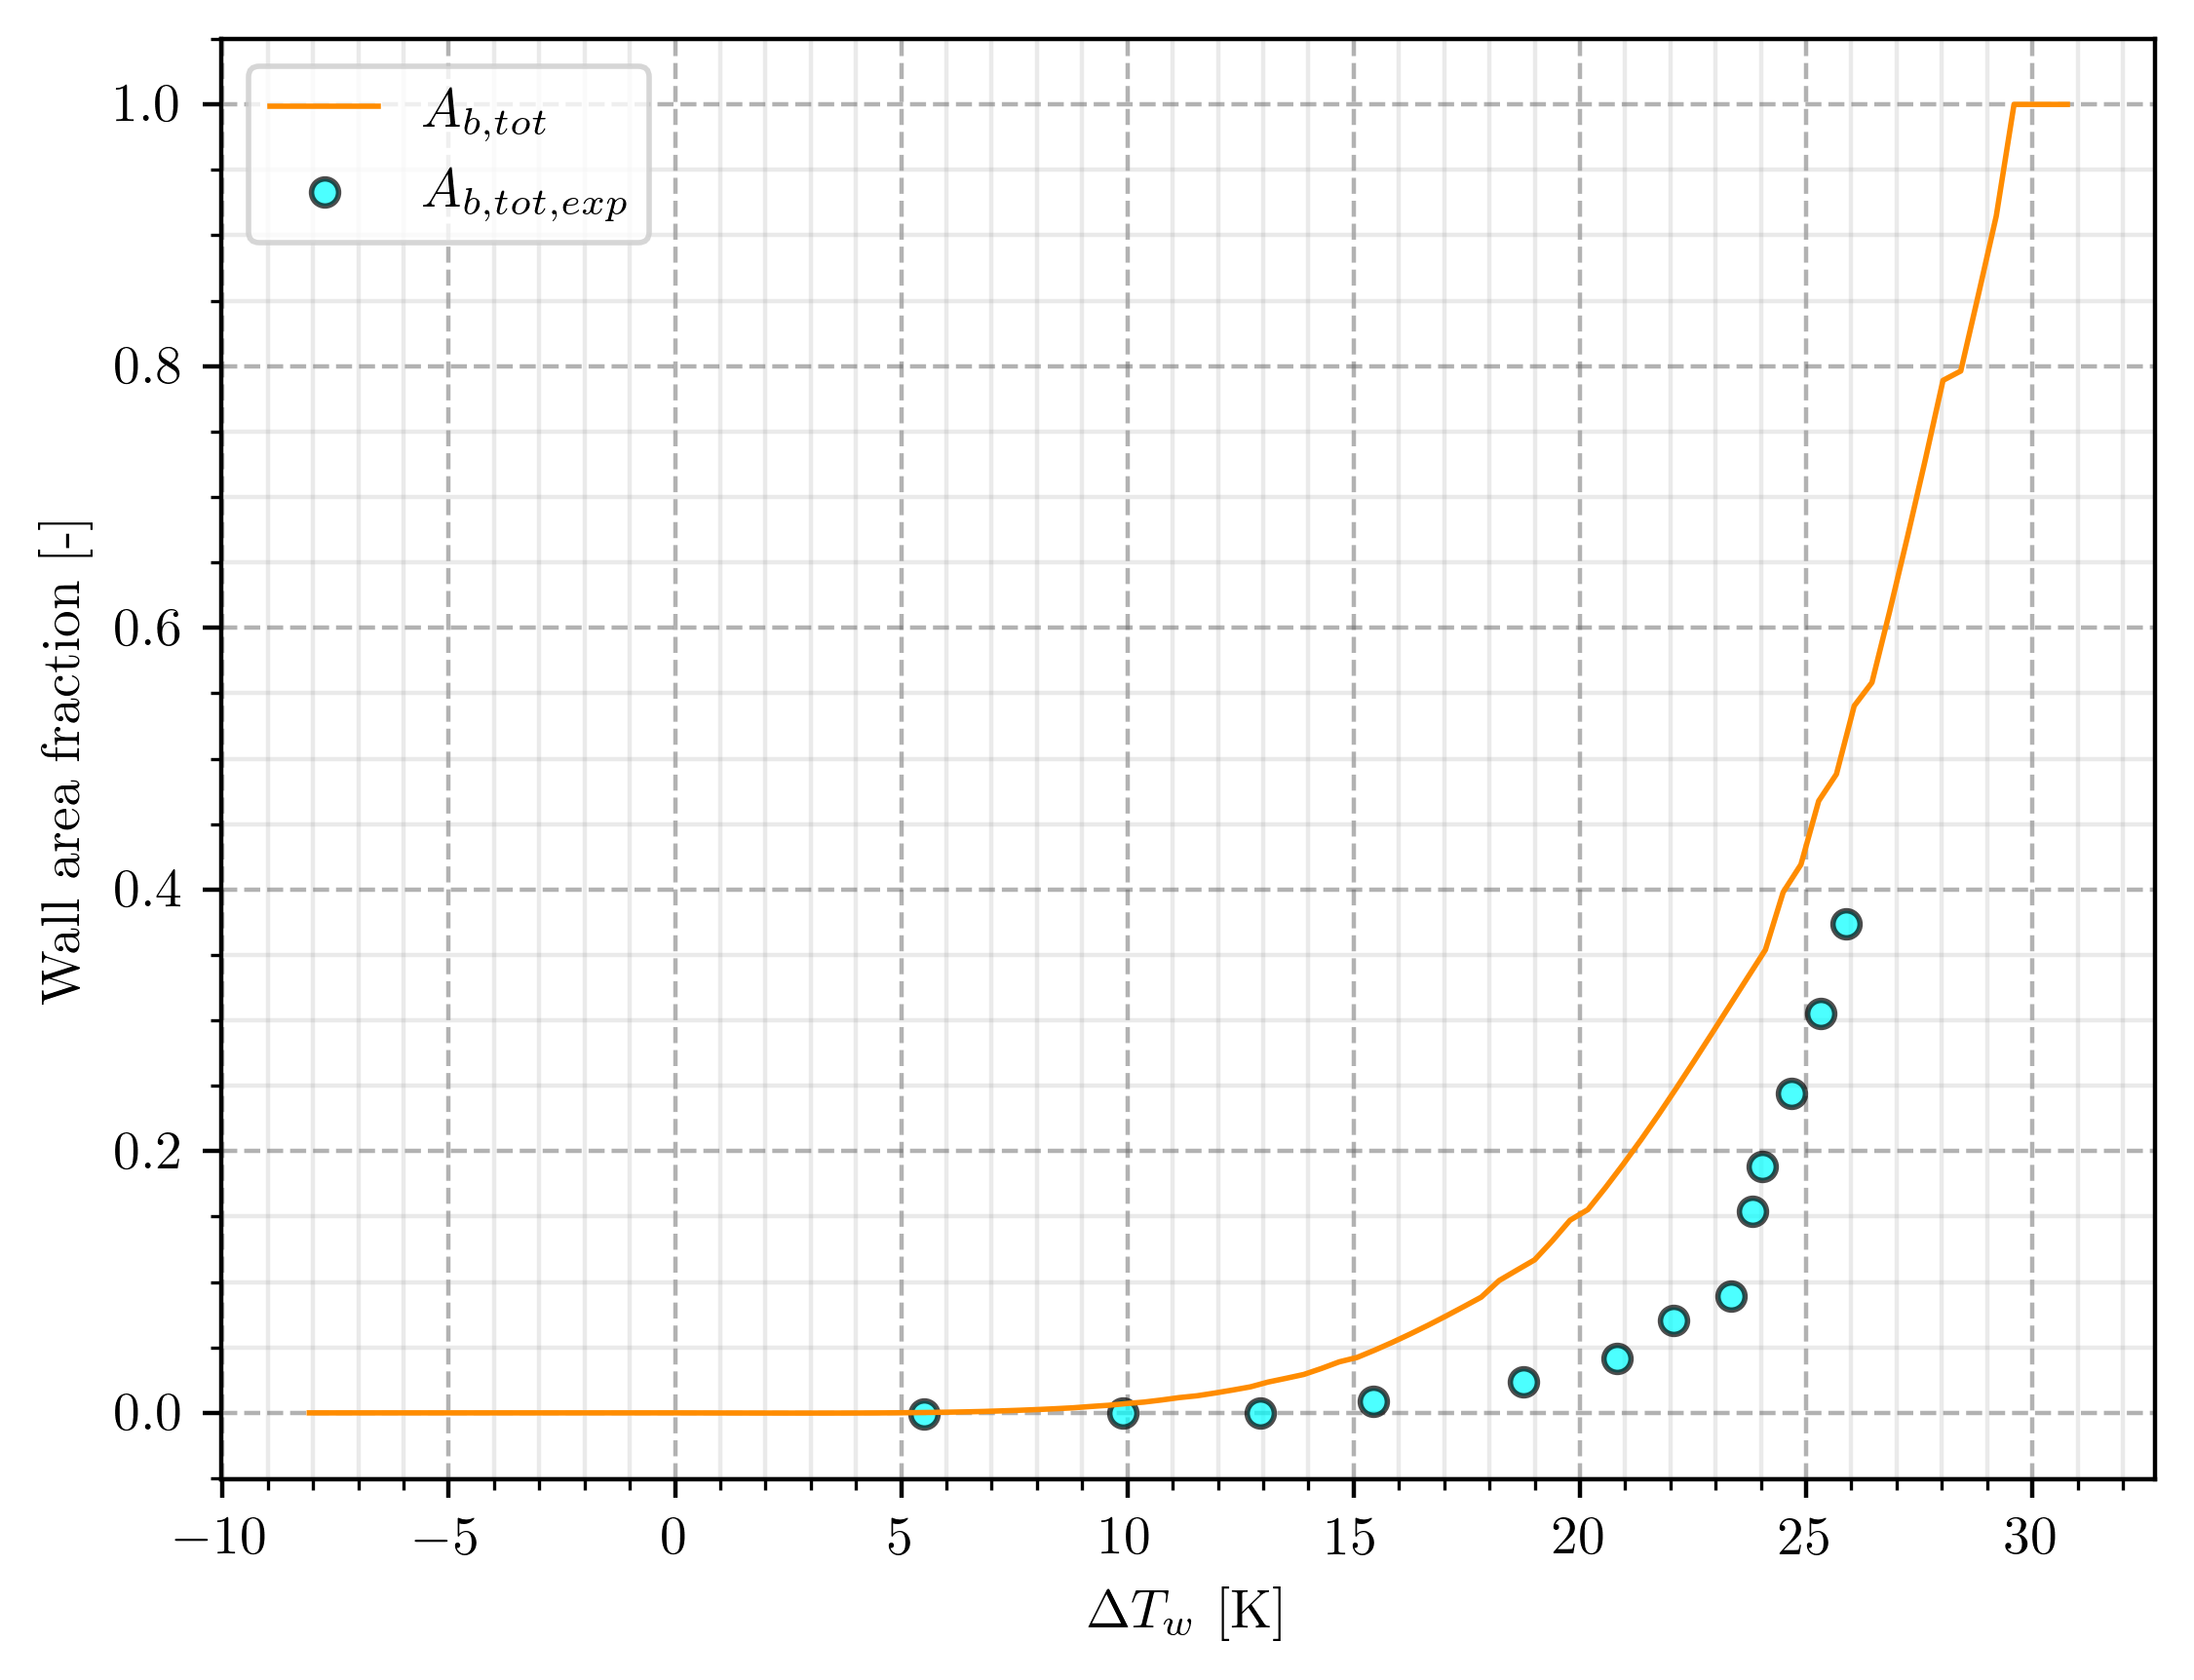
\includegraphics[width=0.5\linewidth]{img/HFP/fullcomp_Koss/Abub_tot_G2000.png}
}
\caption{Comparison of average area visited by a bubble and total wall fraction area impacted by bubbles (footprint or transient conduction).}
\label{fig:fullkoss_area}
\end{figure}

\npar

On Figure \ref{fig:fullkoss_length}, we indicatively show the values of sliding length $l_{sl}$, departure diameter $R_{d}$ and sliding diameter $R_{sl}$ when sliding over $l_{sl}$. The small values of $R_{d}$ are coherent with nearly immediate departure by sliding, with sliding radiuses close to $0.1$ mm.


\begin{figure}[!h]
\centering
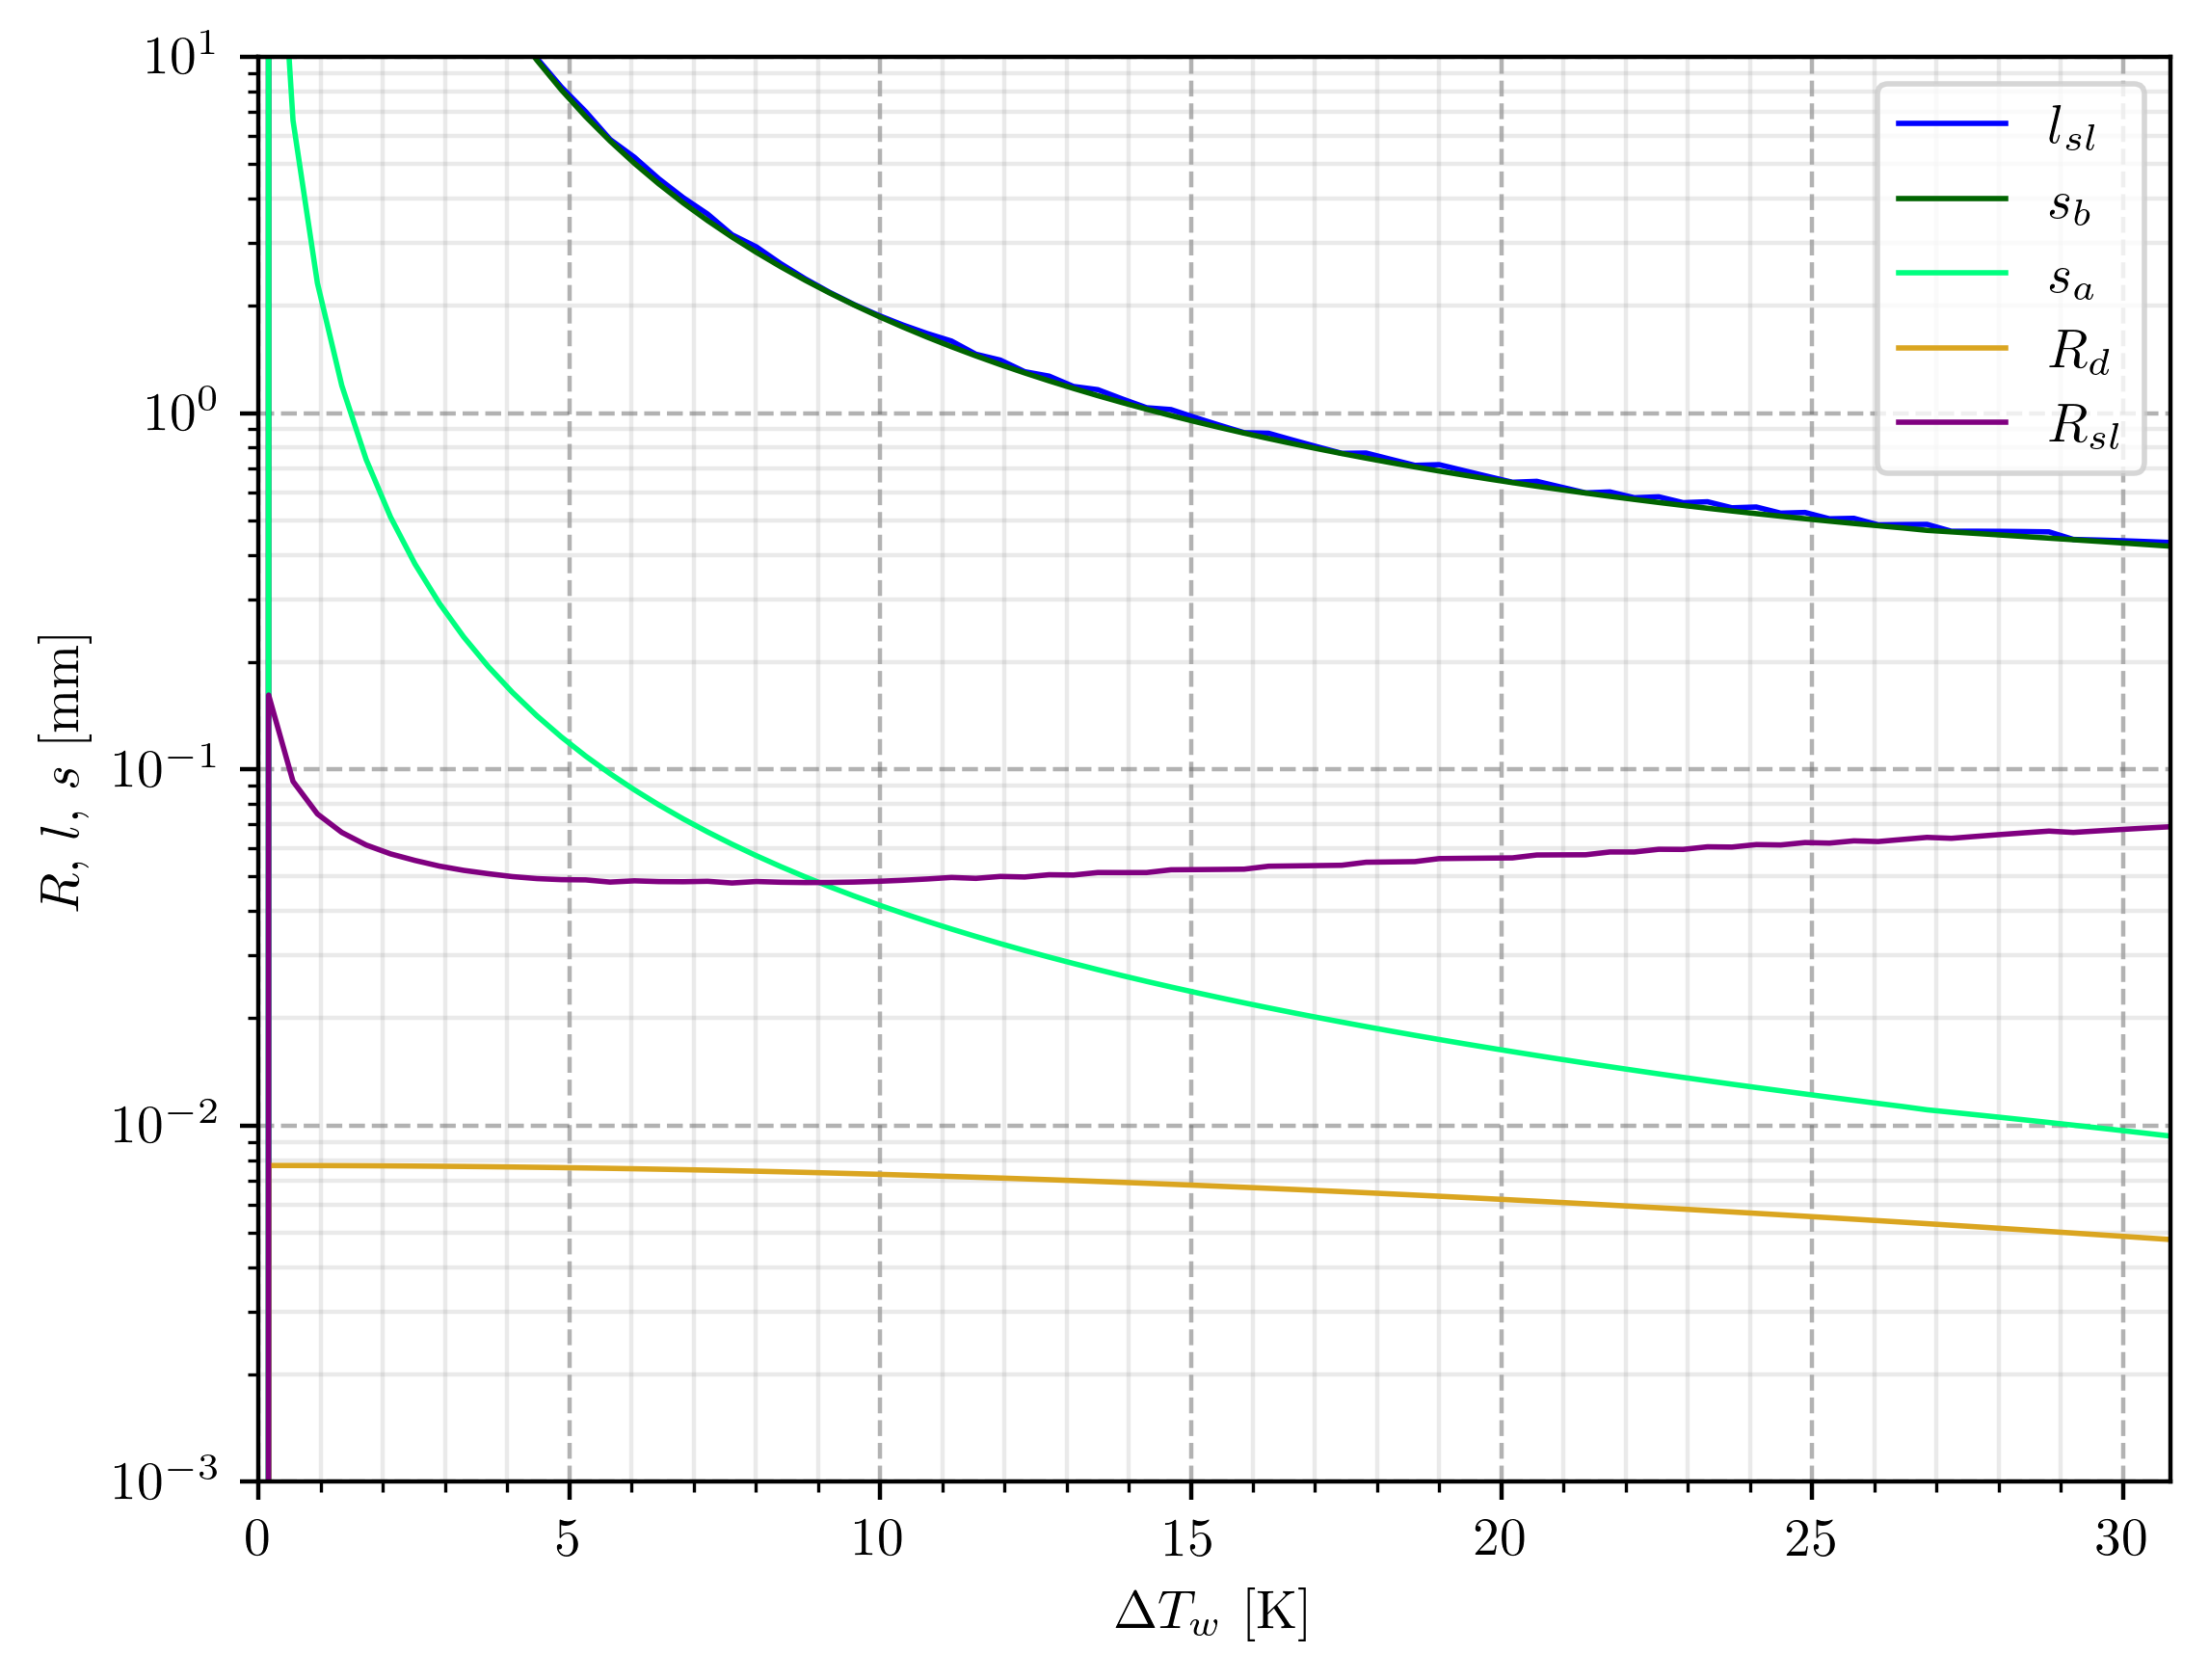
\includegraphics[width=0.5\linewidth]{img/HFP/fullcomp_Koss/length_G2000.png}
\caption{Comparison of average area visited by a bubble and total wall fraction area impacted by bubbles (footprint or transient conduction).}
\label{fig:fullkoss_length}
\end{figure}



\subsection{Flux Proportions and Wall Superheat}

Figure \ref{fig:fullkoss_hfp} finally compares the fraction of single-phase convection and quenching over the total heat flux $\phi_{w}$ along with the boiling curve. The evolution of the single-phase flux reasonably agrees with the experiment and becomes 0 at a superheat similar to the measurement. However, the quenching heat flux is logically overestimated due to the significant overestimation of the area visited by a single bubble.

\npar

On the other hand, the boiling curve is pretty well predicted except for the last experimental measurement where an increase in wall temperature starts, which could correspond to conditions close to the CHF that can't yet be detected by the HFP model.

\begin{figure}[!h]
\subfloat[Single bubble area]{
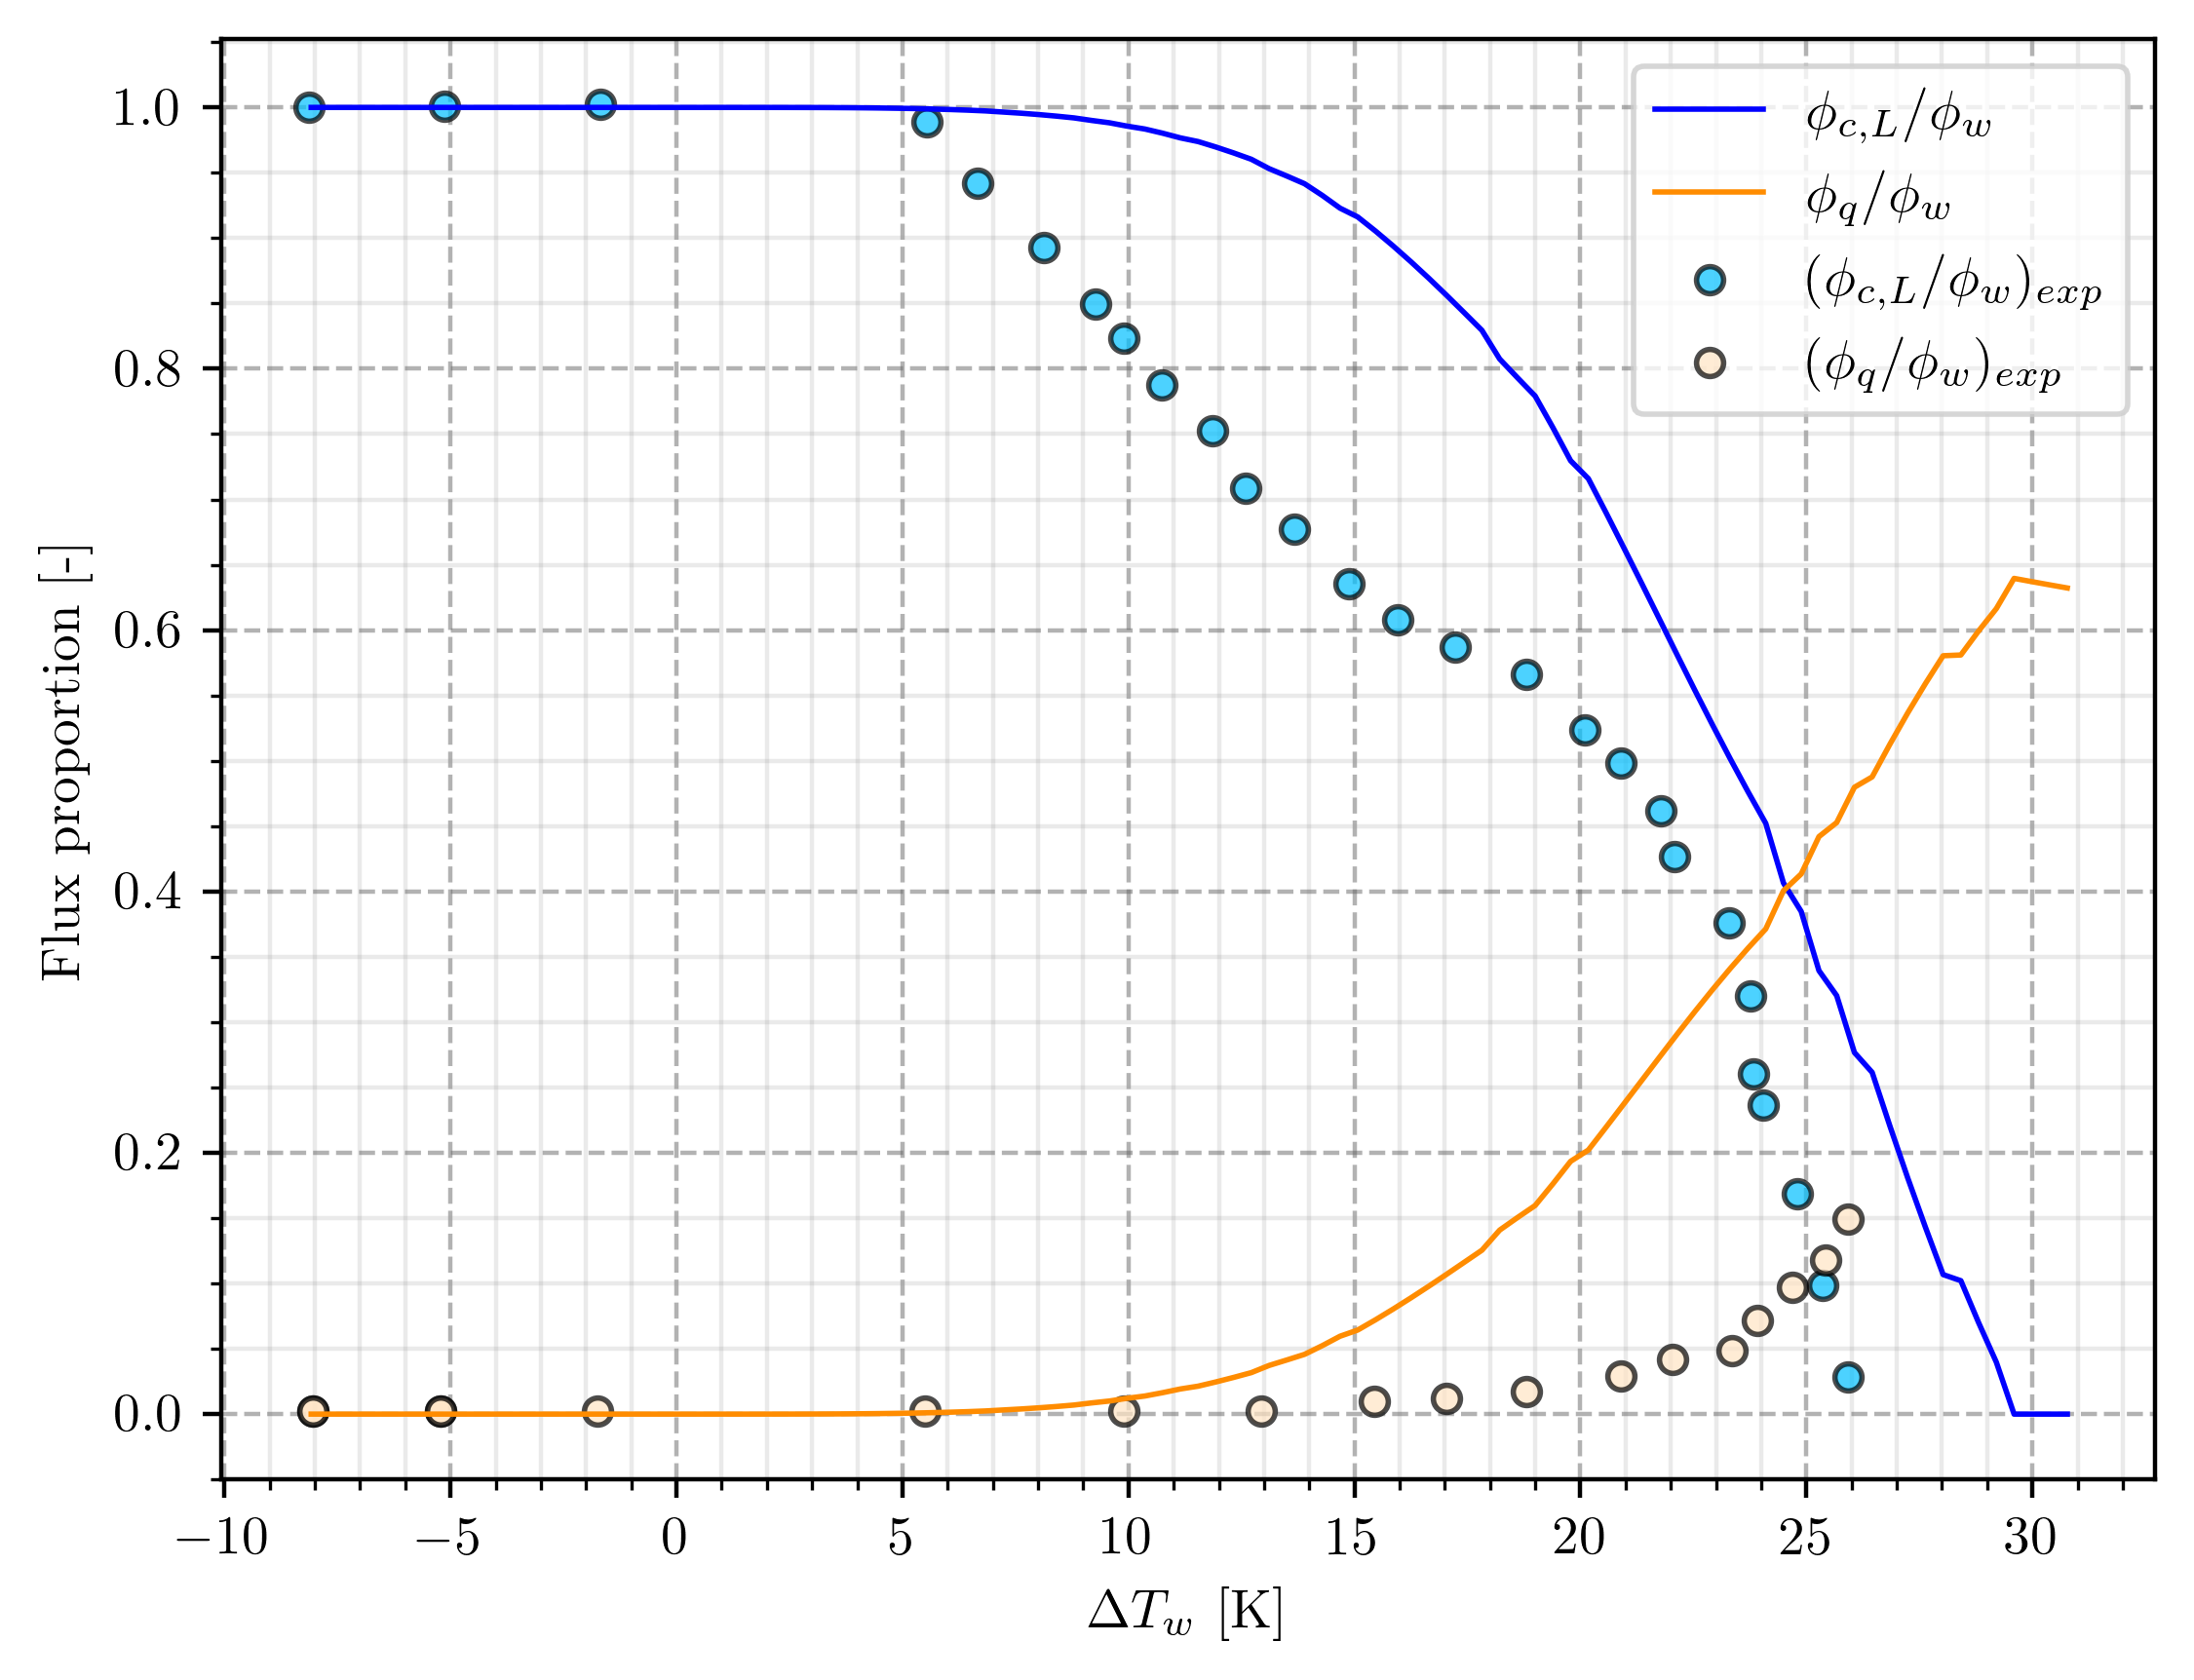
\includegraphics[width=0.5\linewidth]{img/HFP/fullcomp_Koss/hfp_G2000.png}
}
\subfloat[Total wall area impacted by bubbles]{
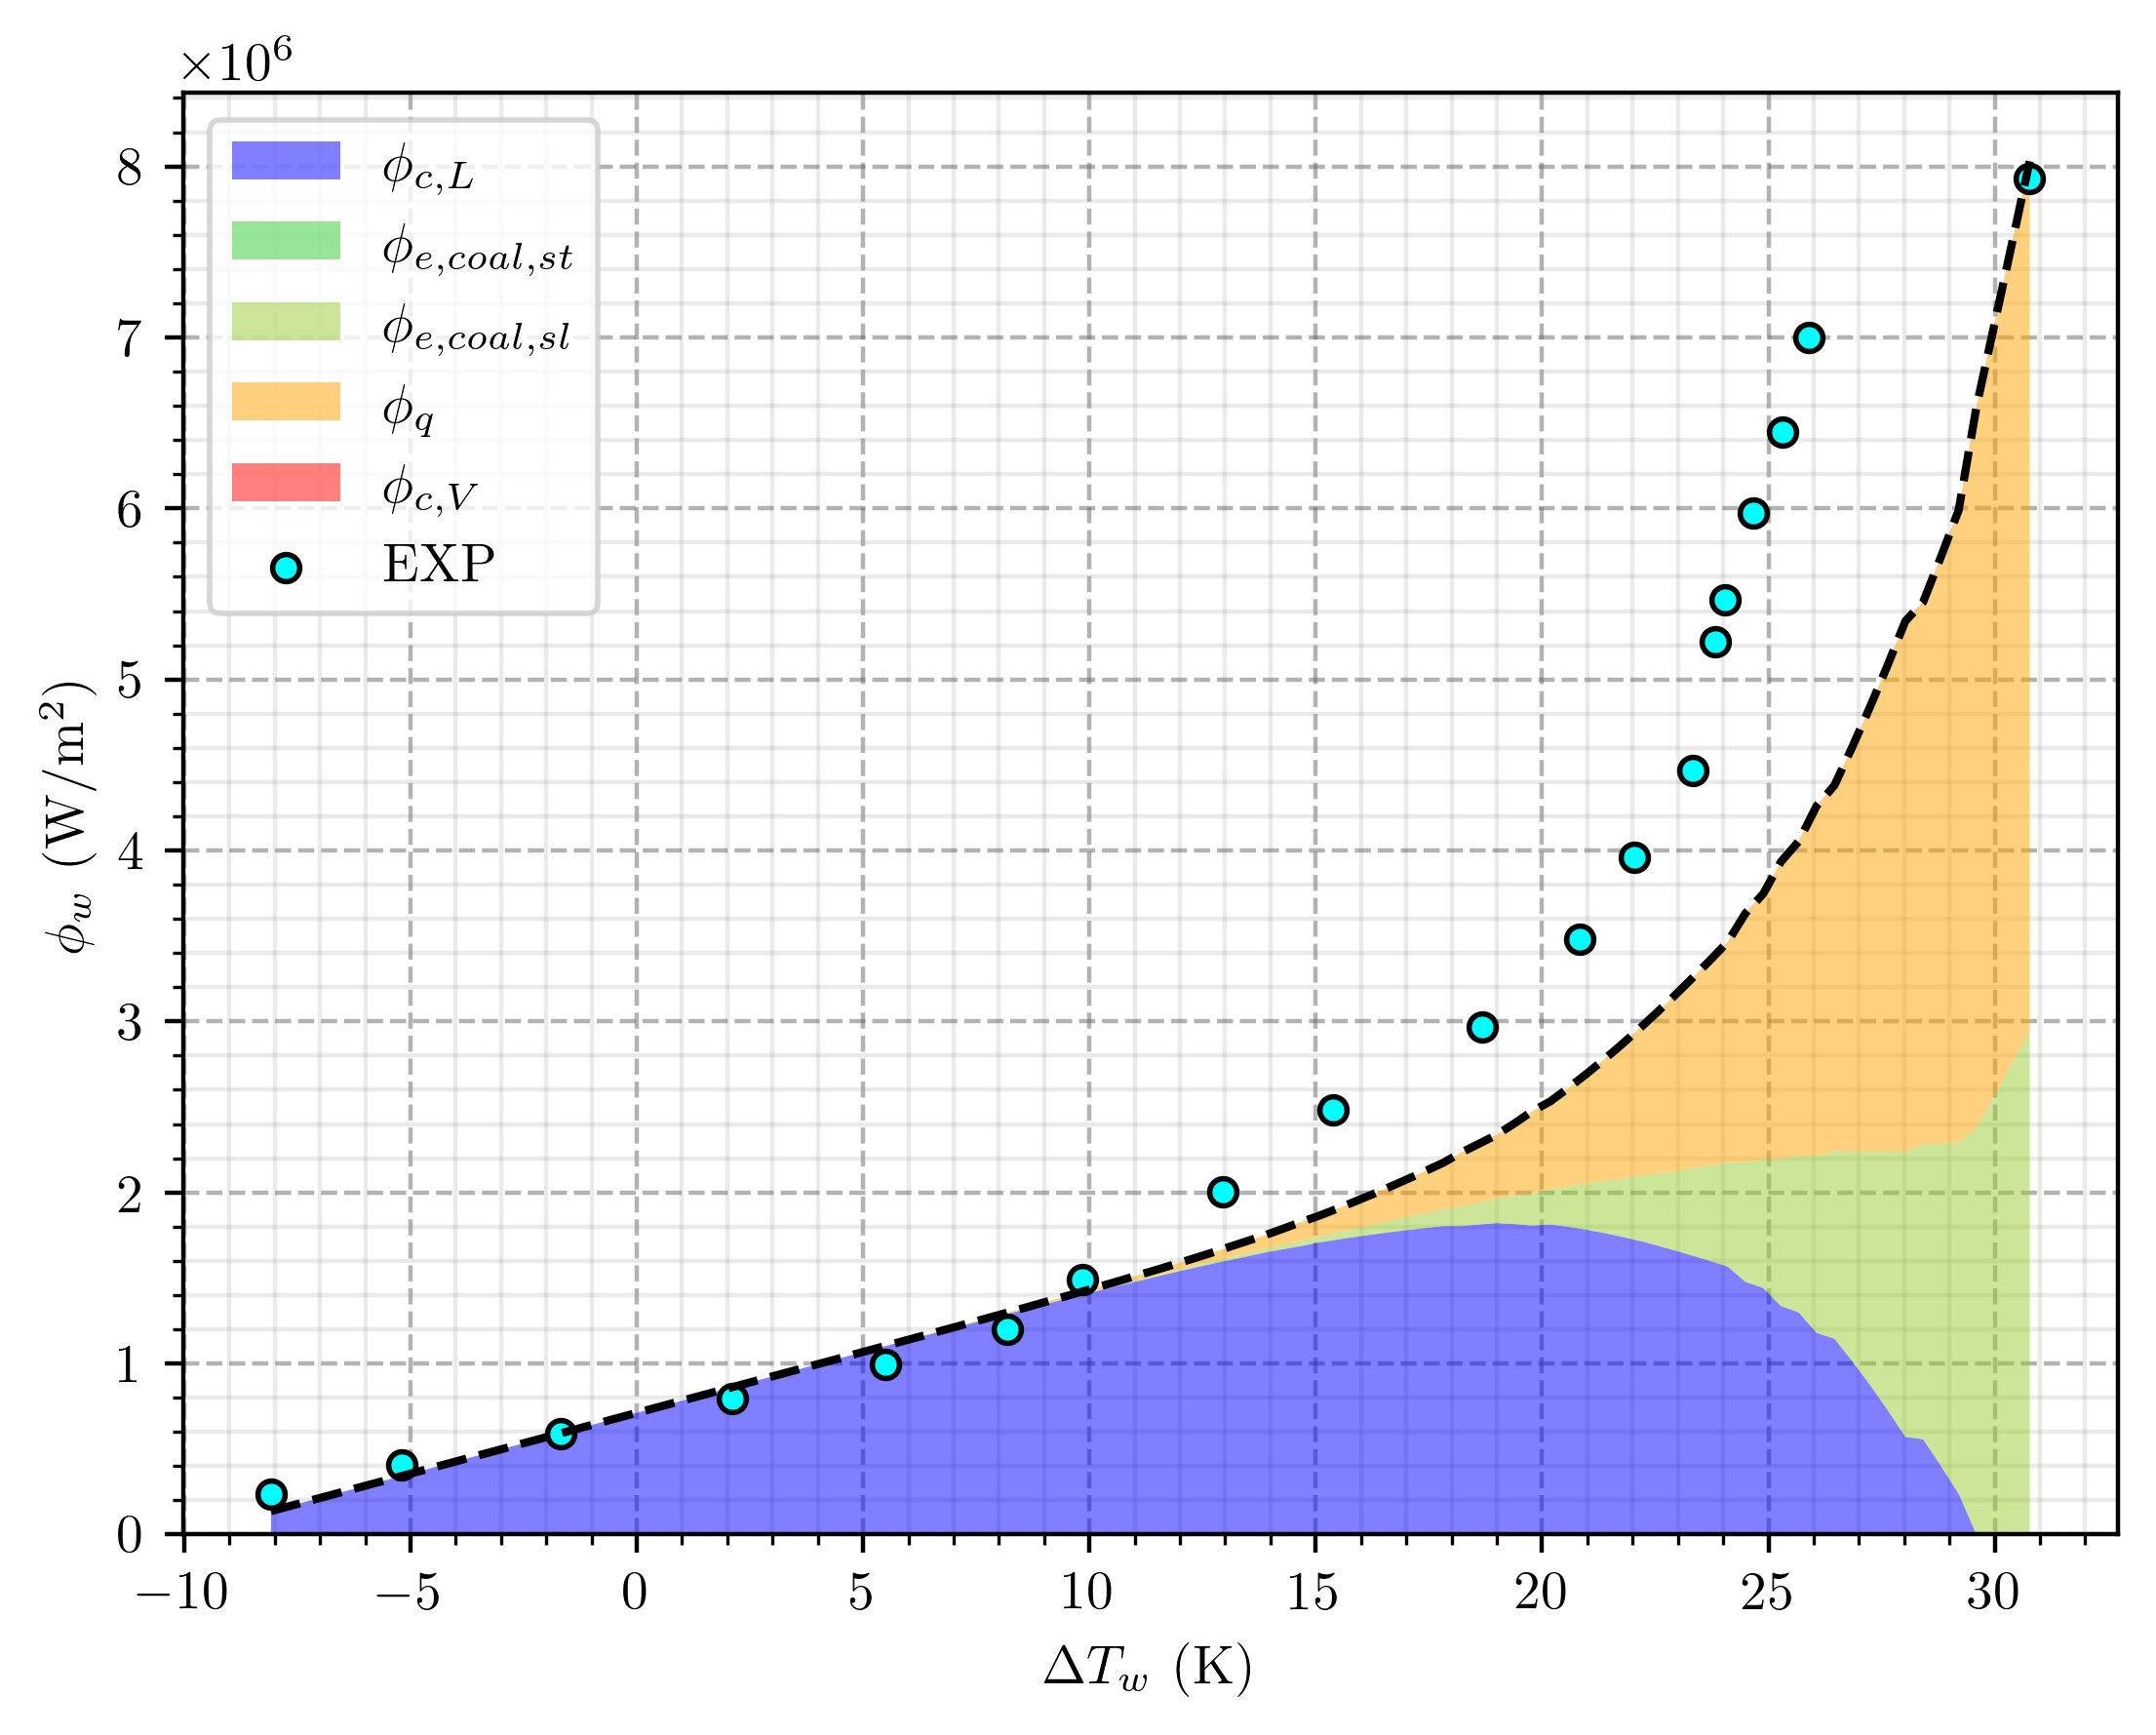
\includegraphics[width=0.5\linewidth]{img/HFP/fullcomp_Koss/boil_curve_G2000.png}
}
\caption{Comparison of average area visited by a bubble and total wall fraction area impacted by bubbles (footprint or transient conduction).}
\label{fig:fullkoss_hfp}
\end{figure}




\section{Wall Temperature Predictions}


In this section, we want to evaluate the model's capability to predict wall temperature in boiling regimes for different flow conditions. To do so, we gather boiling curves data from the literature for water that covers a large range of flow conditions as detailed in Table \ref{tab:exp_data_HFP}.


\begin{table}[h!]

%\begin{changemargin}{-1cm}{0cm}

\noindent\makebox[\textwidth]{

\scriptsize
\centering
\begin{tabular}{p{20mm}|c c c c c c c c} 
Author & $D_{h}$ [mm] & $P$ [bar] & $G_{L}$ [$\debm$] & $\Delta T_{L}$ [K] & $\phi_{w}$ [MW/m\up{2}] & $T_{sat}-T_{w}$ [K] &$N_{mes}$ [-] \\
\hline
\\

Kossolapov \cite{kossolapov_experimental_2021} \newline (2021) & 12 & 1.12 - 75.8 & 500 - 2000 & 10 & 0.1 - 0.6  & 0.22 - 9.5 & 12 \\

Jens-Lottes \cite{jens_analysis_1951} \newline (1951) & 5.74 & 137.9 & 2617.5 & 53.3 - 92.2 & 0.91 - 2.37 & 0.33 - 44.1 & 15 \\

Kennel \cite{kennel_local_1949} \newline (1948) & 4.3 - 13.2 & 2 - 6.2 & 284 - 10~577 & 11.1 - 83.3 & 0.035 - 1.89 & 0.35 - 69 & 52 \\
\hline
\end{tabular}
}
\caption{Experimental data range of wall temperature measurements from the single-phase part of boiling curves.}
\label{tab:exp_data_HFP}
\end{table}


\subsection{Kennel Data}

\begin{figure}[!h]
\centering
\subfloat[Kurul \& Podowski]{
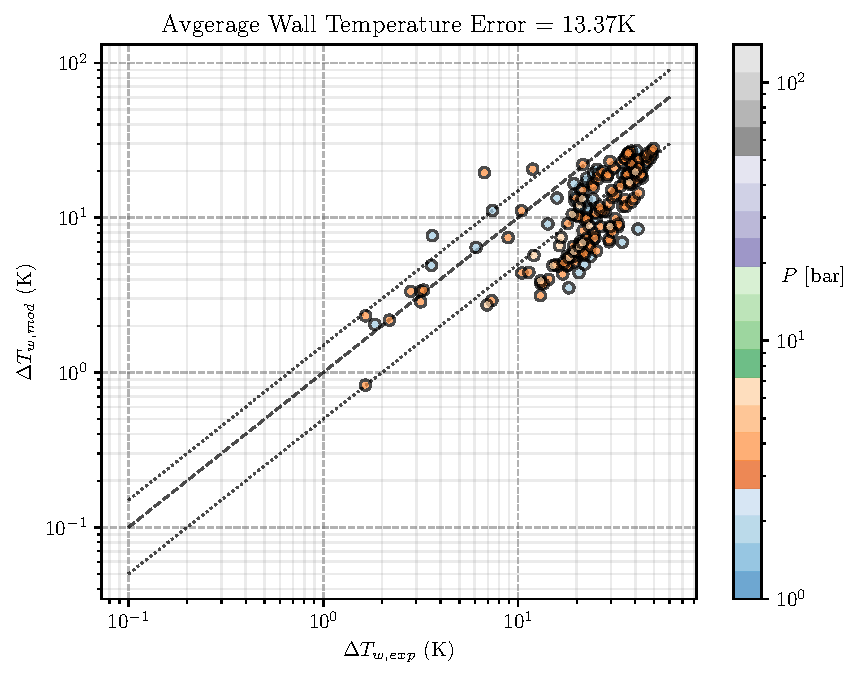
\includegraphics[width=0.5\linewidth]{img/HFP/kennel/KP_Kennel.pdf}
}
\subfloat[Basu]{
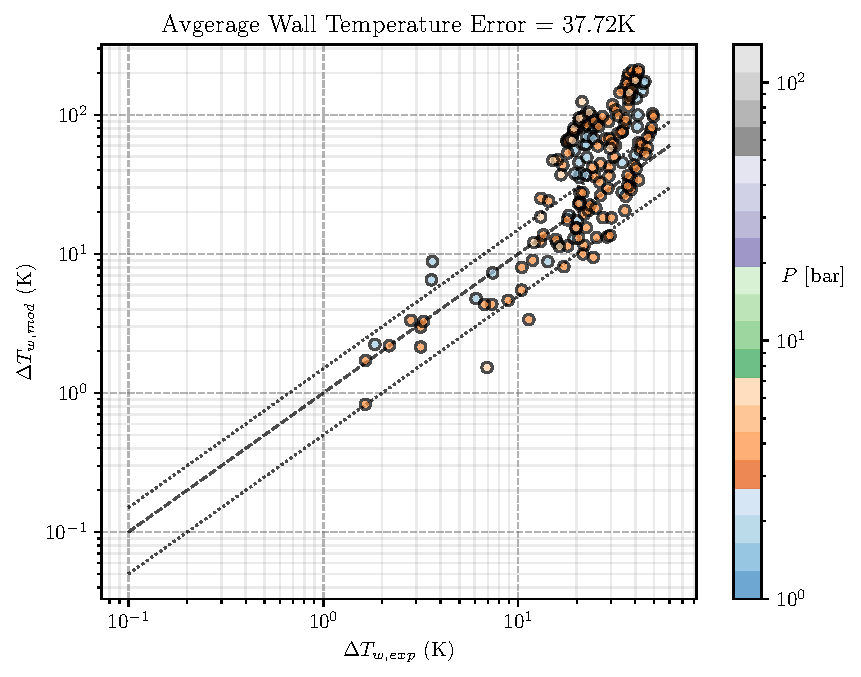
\includegraphics[width=0.5\linewidth]{img/HFP/kennel/Basu_Kennel.pdf}
}
\\
\subfloat[Kommajosyula]{
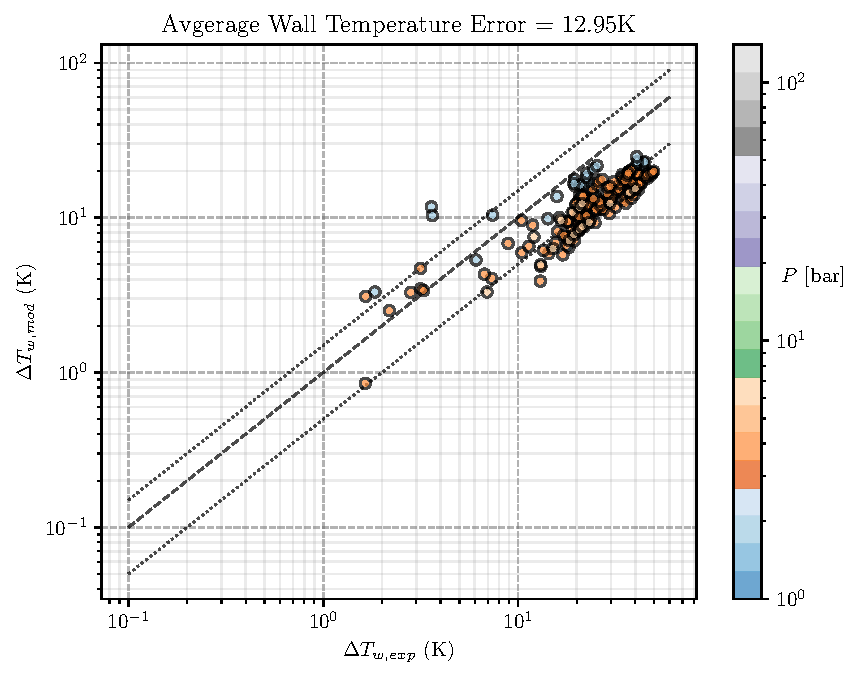
\includegraphics[width=0.5\linewidth]{img/HFP/kennel/Komma_Kennel.pdf}
}
\subfloat[New Model]{
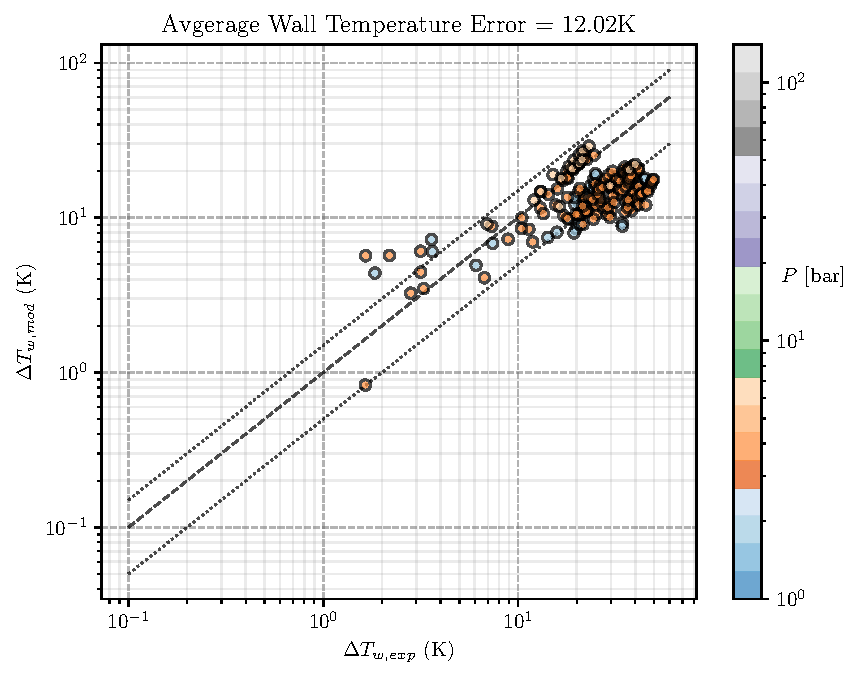
\includegraphics[width=0.5\linewidth]{img/HFP/kennel/NM_Kennel_t50_K05_dt5.pdf}
}

\caption{Wall temperature predictions achieved by the different HFP models on Kennel data. $\theta = 50 \degree$}
\label{fig:HFP_kennel}
\end{figure}


\subsection{Kossolapov Data}

\begin{figure}[!h]
\centering
\subfloat[Kurul \& Podowski]{
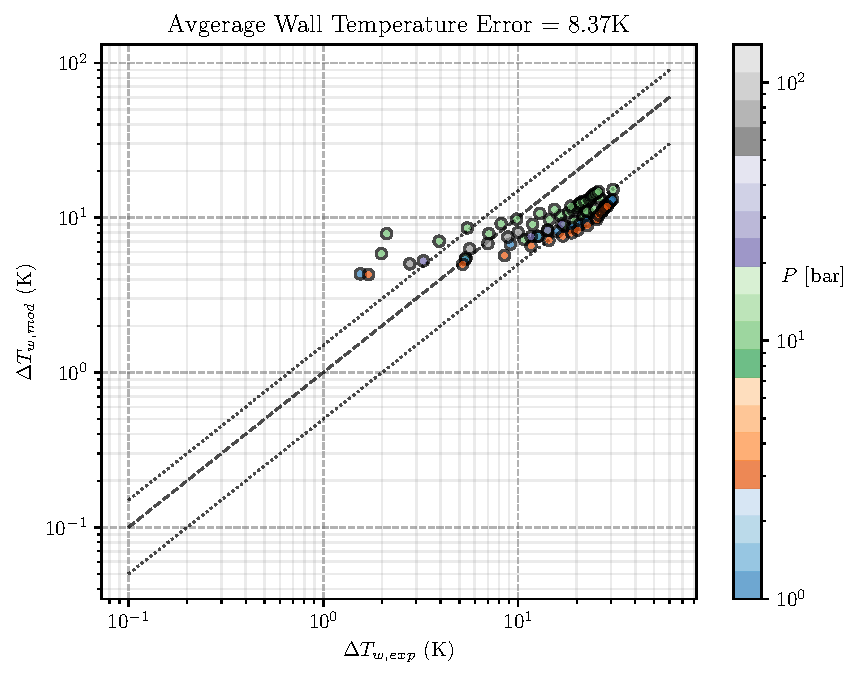
\includegraphics[width=0.5\linewidth]{img/HFP/koss/KP_Kossolapov.pdf}
}
\subfloat[Basu]{
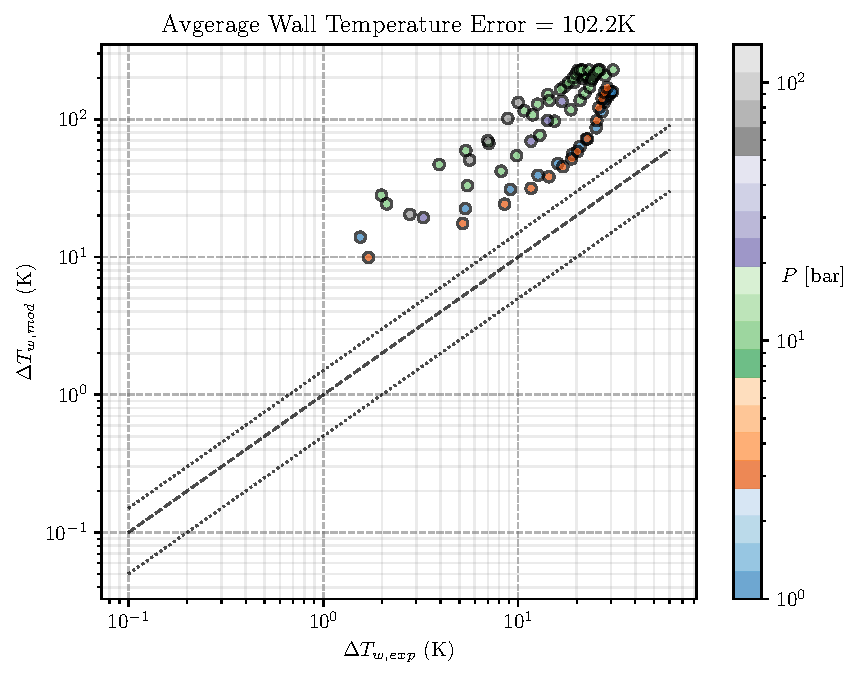
\includegraphics[width=0.5\linewidth]{img/HFP/koss/Basu_Kossolapov.pdf}
}
\\
\subfloat[Kommajosyula]{
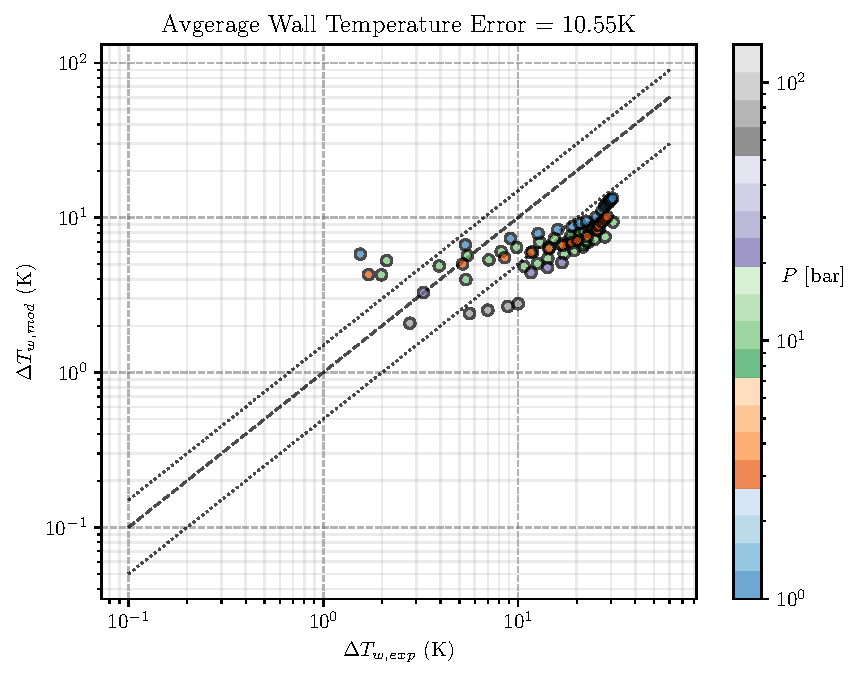
\includegraphics[width=0.5\linewidth]{img/HFP/koss/Komma_Kossolapov.pdf}
}
\subfloat[New Model]{
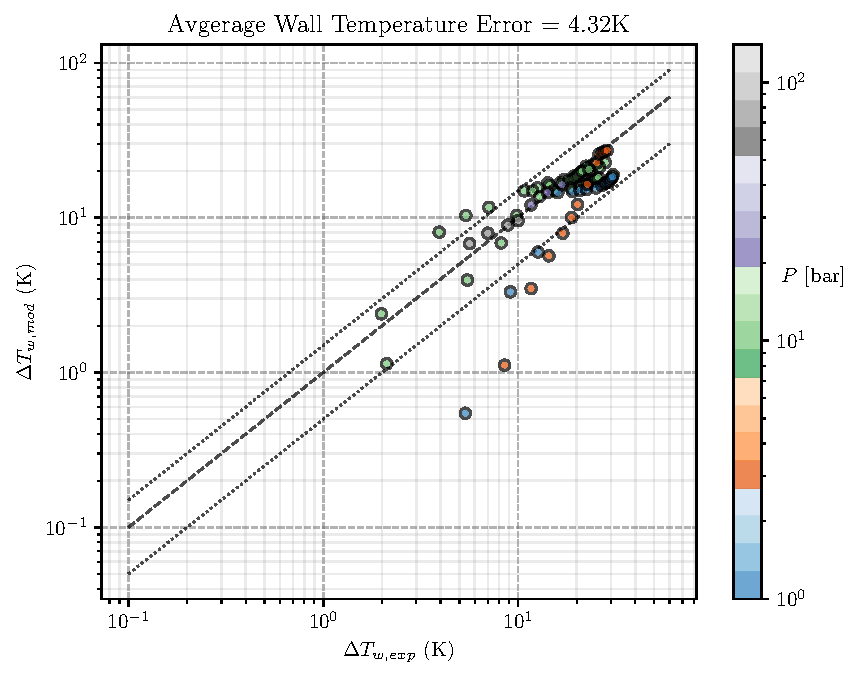
\includegraphics[width=0.5\linewidth]{img/HFP/koss/NM_Kossolapov.pdf}
}

\caption{Wall temperature predictions achieved by the different HFP models on Kossolapov data. $\theta = 85\degree$}
\label{fig:HFP_koss}
\end{figure}



\subsection{Jens-Lottes Data}

\begin{figure}[!h]
\centering
\subfloat[Kurul \& Podowski]{
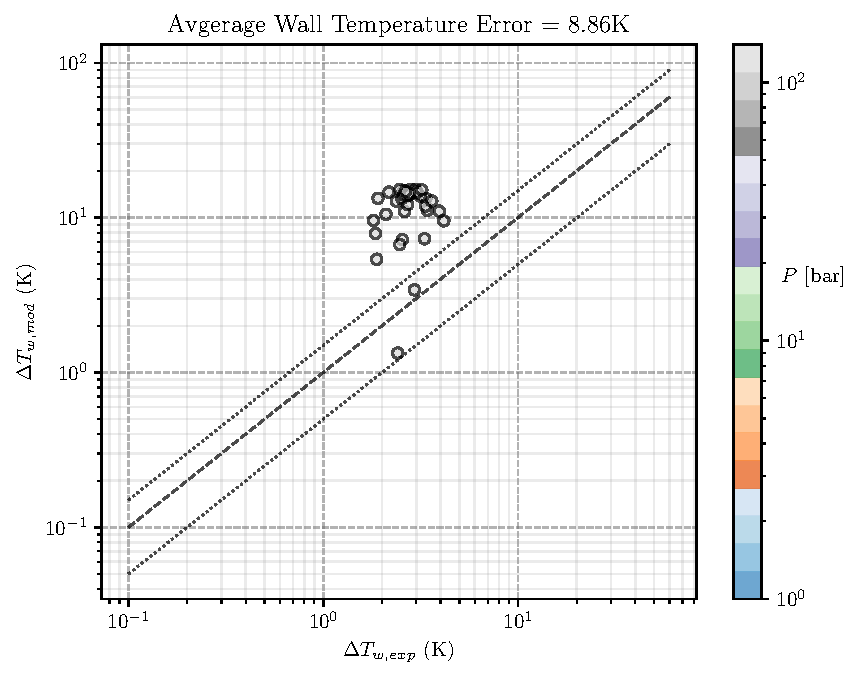
\includegraphics[width=0.5\linewidth]{img/HFP/jens/KP_Jens.pdf}
}
\subfloat[Basu]{
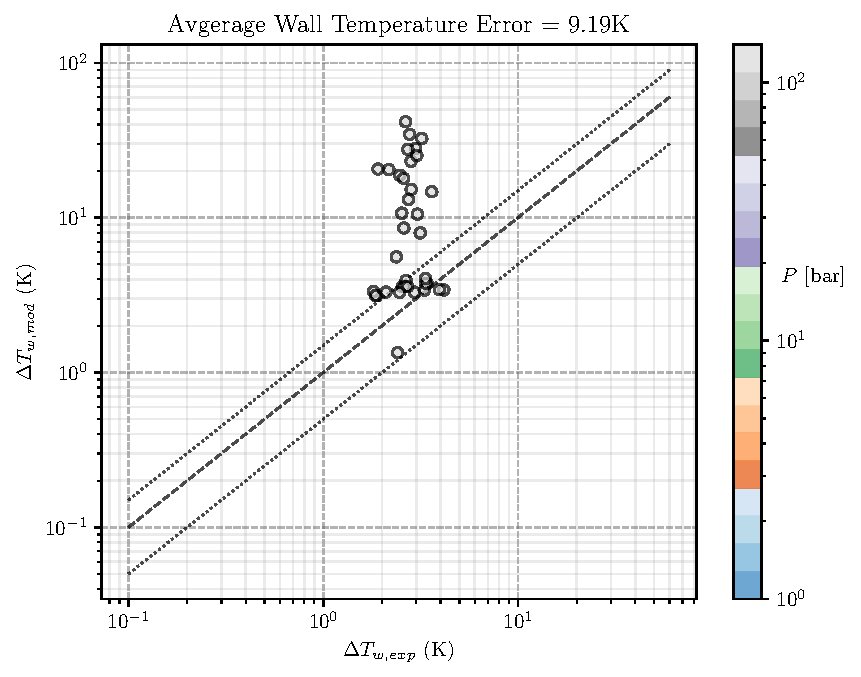
\includegraphics[width=0.5\linewidth]{img/HFP/jens/Basu_Jens.pdf}
}
\\
\subfloat[Kommajosyula]{
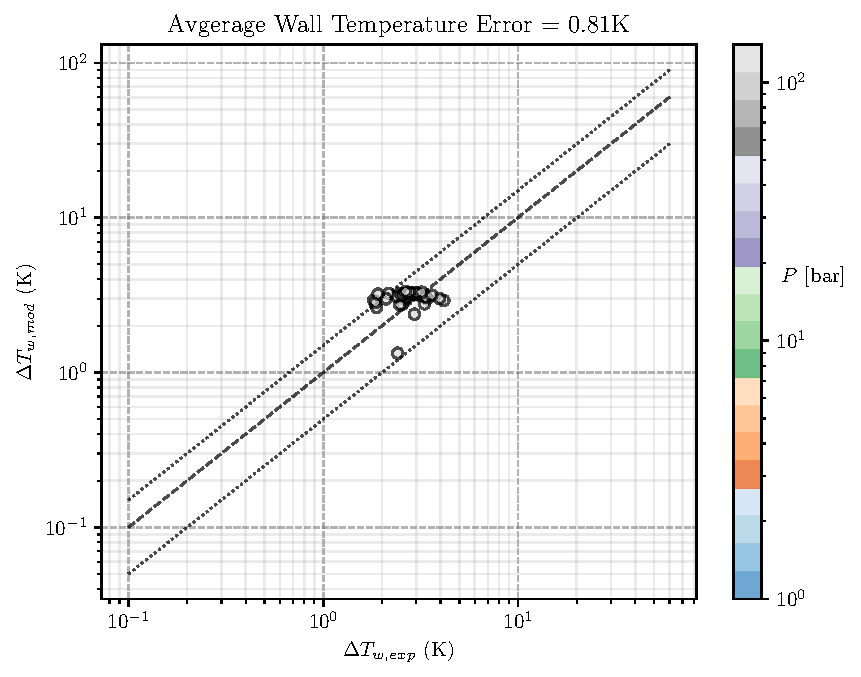
\includegraphics[width=0.5\linewidth]{img/HFP/jens/Komma_Jens.pdf}
}
\subfloat[New Model]{
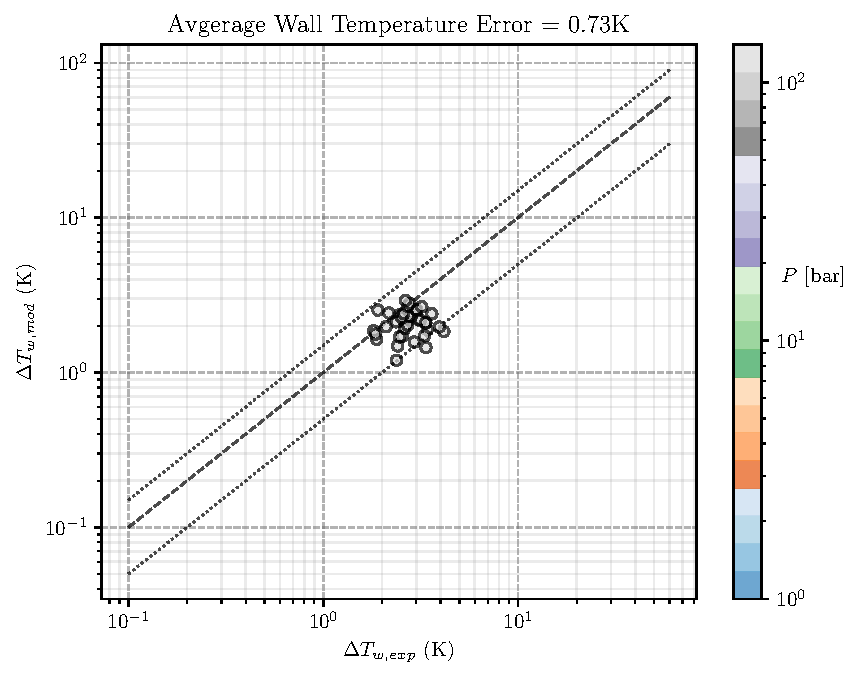
\includegraphics[width=0.5\linewidth]{img/HFP/jens/NM_Jens.pdf}
}

\caption{Wall temperature predictions achieved by the different HFP models on Jens data. $\theta = 20\degree$}
\label{fig:HFP_kennel}
\end{figure}



\section{Validation DEBORA Experiment}


We 

